\documentclass[14pt,a4paper,oneside,openany]{extreport}
\pdfminorversion=7
\usepackage[T1]{fontenc}
\usepackage[utf8]{inputenc}
\usepackage[numbers,sort&compress]{natbib}
\usepackage[english]{babel}
\usepackage{lmodern,microtype}
\usepackage[a4paper,left=3cm,right=2.5cm,top=2.5cm,bottom=2.5cm,headheight=15pt]{geometry}
\usepackage{amsmath,amssymb,amsthm,mathtools,bm}
\usepackage{graphicx,booktabs,array,tabularx,longtable,multirow}
\usepackage{xcolor,setspace,fancyhdr,enumitem,titlesec}
\usepackage{needspace,etoolbox}
\usepackage{tikz}
\usetikzlibrary{arrows.meta,positioning,fit,calc,shapes.geometric}
\usepackage[font=small,labelfont=bf]{caption}
\usepackage{subcaption,float,placeins}
\usepackage[hidelinks,breaklinks]{hyperref}
\usepackage{bookmark}
\hypersetup{pdftitle={Safe Drone Navigation under Disturbance Shifts},pdfauthor={Salem Fradi},pdfsubject={SupCom final year internship report 2026}}
\definecolor{navy}{HTML}{18334F}
\definecolor{teal}{HTML}{067C82}
\definecolor{lightblue}{HTML}{DBE6F0}
\setstretch{1.10}
\setlength{\parindent}{1.25em}
\setlength{\parskip}{0.15em}
\setlength{\emergencystretch}{3em}
\setlength{\textfloatsep}{16pt plus 2pt minus 2pt}
\setlength{\floatsep}{14pt plus 2pt minus 2pt}
\setlist{itemsep=2pt,topsep=5pt,leftmargin=1.8em}
\titleformat{\chapter}[display]{\normalfont\LARGE\bfseries\raggedright\hyphenpenalty=10000}{\large Chapter \thechapter}{8pt}{}
\titlespacing*{\chapter}{0pt}{-12pt}{22pt}
\titleformat{\section}{\large\bfseries\raggedright\hyphenpenalty=10000}{\thesection}{.7em}{}
\titleformat{\subsection}{\normalsize\bfseries\raggedright\hyphenpenalty=10000}{\thesubsection}{.7em}{}
\titleformat{\subsubsection}{\normalsize\bfseries\raggedright\hyphenpenalty=10000}{}{0pt}{}
\titlespacing*{\subsubsection}{0pt}{12pt}{6pt}
\setcounter{tocdepth}{1}
\renewcommand{\thechapter}{\Roman{chapter}}
\newcommand{\introsection}[1]{\section*{#1}\phantomsection\addcontentsline{toc}{section}{#1}}
\setcounter{secnumdepth}{2}
\makeatletter
\renewcommand*{\l@section}{\@dottedtocline{1}{1.5em}{3em}}
\patchcmd{\l@chapter}{1.5em}{2.3em}{}{\errmessage{Chapter entry width patch failed}}
\renewcommand*{\l@figure}{\@dottedtocline{1}{1.5em}{3em}}
\let\l@table\l@figure
\let\report@chapterentry\l@chapter
\renewcommand*{\l@chapter}[2]{\Needspace{3\baselineskip}\report@chapterentry{#1}{#2}}
\makeatother
\pagestyle{fancy}
\fancyhf{}
\fancyhead[L]{\small Sup'Com}
\fancyhead[R]{\small Salem Fradi}
\fancyfoot[C]{\thepage}
\renewcommand{\headrulewidth}{.3pt}
\fancypagestyle{plain}{\fancyhf{}\fancyfoot[C]{\thepage}\renewcommand{\headrulewidth}{0pt}}
\newtheorem{theorem}{Theorem}[chapter]
\newtheorem{proposition}[theorem]{Proposition}
\newtheorem{lemma}[theorem]{Lemma}
\theoremstyle{definition}
\newtheorem{definition}[theorem]{Definition}
\newtheorem{assumption}[theorem]{Assumption}
\theoremstyle{remark}
\newtheorem{remark}[theorem]{Remark}
\newcommand{\R}{\mathbb R}
\newcommand{\E}{\mathbb E}
\newcommand{\Prob}{\mathbb P}
\newcommand{\norm}[1]{\left\lVert#1\right\rVert}
\newcommand{\pos}[1]{\left[#1\right]_+}
\newcommand{\cvar}{\operatorname{CVaR}}
\newcommand{\clip}{\operatorname{clip}}
\DeclareMathOperator*{\argmin}{arg\,min}
\DeclareMathOperator*{\argmax}{arg\,max}
\newcolumntype{Y}{>{\raggedright\arraybackslash}X}
\begin{document}
\selectlanguage{english}
\hypersetup{pageanchor=false}
\begin{titlepage}
\thispagestyle{empty}\fontsize{12}{14.5}\selectfont
\begin{center}

\includegraphics[width=6.2cm]{figures/supcom_logo.pdf}
\end{center}
\vspace{.6cm}
\hrule
\begin{center}
\vspace{.5cm}
{\fontsize{14.4}{18}\selectfont\itshape Telecommunications Engineering Program}\\[.6cm]
{\fontsize{20.74}{25}\selectfont\bfseries Final-Year Project Report}\\[.5cm]
{\fontsize{14.4}{18}\selectfont Project Title}\\[.3cm]
{\fontsize{20.74}{25}\selectfont\bfseries Safe Drone Navigation\\[.15cm]Under Disturbance Shifts}\\[.35cm]
{\fontsize{14.4}{18}\selectfont\bfseries Reinforcement Learning, Safety and\\Disturbance Rejection}\\[.5cm]
{\fontsize{14.4}{18}\selectfont\itshape Prepared by}\\[.15cm]
{\fontsize{17.28}{22}\selectfont\bfseries Salem Fradi}\\[.5cm]
{\fontsize{14.4}{18}\selectfont\itshape Supervisors}\\[.2cm]
\begin{tabular}{ll}
Hakim Ghazzai & KAUST\\[.15cm]
Mohamed Siala & Sup'Com
\end{tabular}\\[.5cm]
{\itshape Work proposed and carried in collaboration with}\\[.2cm]

\includegraphics[height=1.15cm]{figures/kaust_logo.pdf}\\[.1cm]
{\bfseries KAUST}\\[.1cm]
{\fontsize{12}{14.5}\selectfont\bfseries King Abdullah University of Science and Technology}\\[.1cm]
{Thuwal, Saudi Arabia}\\[.55cm]
{Internship Period: 1 February--30 July 2026}\\[.25cm]
{Academic Year: 2025--2026}
\end{center}
\vfill
\noindent\colorbox{lightblue}{\parbox{\dimexpr\textwidth-2\fboxsep\relax}{\centering\fontsize{11}{13.6}\selectfont
Higher School of Communication of Tunis\\
\textbf{SUP'COM}\\
2083 Elghazala Communication Technology Park -- Ariana -- Tunisia\\
Tel. +216 70 240 900 -- \url{https://www.supcom.tn}
}}
\end{titlepage}
\hypersetup{pageanchor=true}
\pagenumbering{roman}
\chapter*{Acknowledgements}
\addcontentsline{toc}{chapter}{Acknowledgements}
I would like to express my sincere gratitude to Hakim Ghazzai, my supervisor at KAUST, and Mohamed Siala, my supervisor at Sup'Com, for their guidance throughout this final-year project. Their advice helped me develop the work and present its technical ideas with greater clarity. I am grateful for the time and attention they devoted to supervising this internship.

I thank Hakim Ghazzai for guiding the research carried out in collaboration with KAUST, and Mohamed Siala for his academic supervision at Sup'Com. Bringing these perspectives together helped me connect the engineering foundations of my studies with the demands of a research project in safe robotic navigation.

I also express my appreciation to Sup'Com for the education that prepared me for this work, and to KAUST for the opportunity to carry out the internship. This collaboration provided a valuable setting in which to study reinforcement learning, control barrier functions and disturbance-aware navigation, and to develop greater independence in conducting and communicating research.

Finally, I thank everyone who contributed to the discussions and feedback surrounding this project. Preparing this report has reinforced the importance of examining assumptions carefully, interpreting experimental results with care and acknowledging the limits of what an evaluation can establish. I am grateful for the guidance that supported this learning process.

\clearpage
\chapter*{Abstract}
\addcontentsline{toc}{chapter}{Abstract}
Reinforcement learning has become a central framework for sequential decision making, with achievements ranging from DeepMind's Atari agents and AlphaGo's victory over a Go world champion to the post-training and alignment of large language models. Robotics extends this progress to embodied intelligence, where learned decisions must interact safely with physical environments.

However, strong performance in training or simulation does not ensure reliable behavior during deployment. Disturbances, uncertainty and differences between simulated and real dynamics can lead to unsafe actions. Despite advances in safe reinforcement learning, offline safe reinforcement learning and constrained learning more broadly, enforcing safety during policy execution remains a major challenge. This motivates combining learned decision making with mathematical safety guarantees. Control barrier functions provide a framework for restricting actions to preserve a safe set under stated assumptions.

This report investigates the combination of reinforcement learning and control barrier functions for drone navigation under disturbances. This perspective motivates assessing robustness in IsaacSim for sim2real reasons.

\noindent\textbf{Keywords:} reinforcement learning, embodied intelligence, robotics, control barrier functions, safe navigation, sim2real.

\clearpage{\small\setstretch{1.0}\tableofcontents}
\clearpage\phantomsection\addcontentsline{toc}{chapter}{List of Figures}\listoffigures
\clearpage\phantomsection\addcontentsline{toc}{chapter}{List of Tables}\listoftables
\chapter*{Notation and Abbreviations}
\addcontentsline{toc}{chapter}{Notation and Abbreviations}
\begin{longtable}{@{}p{.21\textwidth}p{.73\textwidth}@{}}
\toprule Symbol & Meaning\\\midrule\endhead
$x,u$ & State and control input\\
$f,g$ & Nominal dynamics and input map\\
$d,\hat d$ & Disturbance and its estimate\\
$p,v$ & Position and translational velocity\\
$V$ & Control Lyapunov function\\
$B$ & Control barrier function\\
$\mathcal U,\mathcal C$ & Admissible input set and safe set\\
$\pi_\theta$ & Policy with parameters $\theta$\\
$J_r,J_c$ & Expected reward and constraint-cost objectives\\
$\lambda$ & Nonnegative constraint multiplier\\
$\varepsilon$ & PPO clipping parameter\\
$\epsilon,\rho$ & Tail probability and Wasserstein ambiguity radius\\
$W_1$ & 1-Wasserstein distance\\
CVaR & Conditional value-at-risk\\
CBF / CLF & Control barrier / Lyapunov function\\
HOCBF & High-order control barrier function\\
CMDP & Constrained Markov decision process\\
IoT / UAV & Internet of Things / unmanned aerial vehicle\\
PID / MPC & Proportional-integral-derivative / model predictive control\\
PPO / RL & Proximal policy optimization / reinforcement learning\\
INDI & Incremental nonlinear dynamic inversion\\
DOB / EMA & Disturbance observer / exponential moving average\\
RMA & Rapid Motor Adaptation\\
DATT & Deep Adaptive Trajectory Tracking\\
LoTF / LoRA & Learning on the Fly / low-rank adaptation\\
\bottomrule
\end{longtable}
Symbols in figures from other publications retain the notation of their authors and are explained in the corresponding discussion.

\clearpage\pagenumbering{arabic}
\chapter*{General Introduction}
\phantomsection\addcontentsline{toc}{chapter}{General Introduction}
\label{ch:context}
\begingroup
\clubpenalty=10000
\introsection{Overview}
Agile quadrotors are increasingly used as mobile Internet-of-Things (IoT) platforms for inspection, monitoring, mapping, and data collection. However, their lightweight structure and operation in open environments make them particularly vulnerable to wind disturbances, which can degrade navigation performance and increase collision risk. Existing work often addresses either disturbance rejection through adaptive control methods such as $\mathcal L_1$ and incremental nonlinear dynamic inversion (INDI), or safety through control barrier functions (CBFs) and data-driven safe reinforcement learning, while comparatively few approaches treat robustness and safety jointly. This report examines how these directions can be combined in a navigation architecture: reinforcement learning supplies task-oriented decisions, while a control-theoretic safety layer restricts the commands applied to the vehicle. The discussion begins with the basic language of dynamical systems, introduces reinforcement learning and constrained policy optimization, and then develops the role of control barrier functions. It closes by reviewing approaches to disturbance rejection and online adaptation. The central motivation is to understand what each component contributes to reliable navigation when the operating conditions differ from those used for training.

Aerial mobility is particularly useful when sensors must reach locations that are difficult to instrument permanently. An inspection vehicle can approach different parts of a structure, while a monitoring mission can revisit selected locations as conditions change. In both cases, mobility links the physical task to information collection: the robot must reach a useful observation position and remain sufficiently well controlled to collect meaningful measurements. Reliability therefore concerns the continuity and quality of the mission as well as the vehicle's motion~\cite{mozaffari2019tutorial,bouhamed2020ddpg}.

\introsection{Background and Motivation}
Agile quadrotors are increasingly deployed as mobile Internet-of-Things (IoT) platforms for infrastructure inspection, environmental sensing, mapping, and data collection~\cite{mozaffari2019tutorial,bouhamed2020ddpg}. In these applications, mission success depends not only on reaching a destination but also on preserving reliable sensing and data acquisition in uncertain environments. A navigation error near an obstacle may interrupt the mission, damage the vehicle or its payload, and leave the collected data incomplete.

Modern quadrotor navigation stacks often combine map-based planning with a low-latency local controller or policy. Mapping and hierarchical planning maintain feasible routes as the environment is explored~\cite{zhou2021fuel}, whereas learning-based navigation can map compact observations directly to control commands~\cite{bouhamed2020ddpg,kaufmann2023champion}. These components address complementary needs, but they also have different failure modes: a planned route may become stale between updates, while a learned policy may extrapolate poorly beyond the conditions represented during training.

Outdoor operation introduces an additional mismatch between commanded and realized motion. Wind, aerodynamic effects, model mismatch, and low-level tracking errors perturb the translational response and can sharply reduce obstacle clearance~\cite{faessler2018drag}. Learned residual models have enabled agile flight in strong winds~\cite{litNeuralFly2022}, while disturbance-observer methods reconstruct external effects from measured motion and incorporate them into robust safety constraints~\cite{wang2023dobcbf,kalaria2024dobcbfrl}. Such methods motivate adaptation during operation, but their assumptions, data requirements, or preselected robustness levels may limit portability across changing conditions.

\introsection{Related Work}
Several learning and control approaches address navigation safety. Constrained policy optimization can include safety requirements during training, although it generally requires substantial interaction data~\cite{litSafePrimalDual2023}. At deployment, control barrier function (CBF) filters evaluate each proposed command against the current safety condition and modify it only when necessary~\cite{litAmes2017,litAmes2019}. CBF-RL exposes the policy to this correction during training through action substitution without changing the RL optimizer~\cite{litCBFRL2026}. Complementary risk-aware planning and filtering methods use conditional value-at-risk (CVaR) to emphasize rare but consequential tail events~\cite{rockafellar2000cvar,hakobyan2022wasserstein,safaoui2024drcvar,chriat2024wcvarcbf}. Wasserstein distributionally robust optimization (DRO) extends this perspective by guarding against mismatch between empirical and operating distributions~\cite{thEsfahani2018,long2024sensor,mandaokar2026druav}. 

A remaining challenge is the gap between training-time disturbance assumptions and deployment-time conditions. A fixed safety margin can restrict useful movement under mild conditions yet leave insufficient clearance when the disturbance becomes stronger. Likewise, a policy that performs well across a training distribution may encounter persistent wind or combinations of conditions that were poorly represented during learning. This motivates examining both the disturbance response of the controller and the assumptions behind its safety mechanism.

The report follows three connected questions. First, how can a policy learn useful navigation behavior from interaction? Second, how can a separate control mechanism restrict commands before they are applied? Third, how can the overall system respond when its nominal motion model becomes inaccurate? These questions distinguish task performance, constraint enforcement, and adaptation while keeping their interaction visible.

The distinction matters in an inspection mission near a wall. A route planner may provide a collision-free reference, yet wind can displace the vehicle from that route. A tracking controller can reduce the displacement, but its transient response may still consume part of the available clearance. A safety filter must therefore reason about the motion that can actually occur, rather than considering the planned path alone. This example motivates the progression from feedback control to learned policies, barrier filtering, and disturbance-aware navigation.

\introsection{Contribution}
Navigation in changing wind calls for a safety margin that follows the robot's actual motion. Long et al. account for uncertainty using updated sensor measurements and state estimates~\cite{long2024sensor}. Their sensor-based construction does not explicitly track a rolling history of disturbance prediction errors. This leaves the adaptation to changing motion mismatch to a separate mechanism. We address this gap by making recent disturbance residuals directly determine the CBF safety margin.

Our approach combines an EMA-inspired disturbance observer with a rolling residual window. The observer captures the recent disturbance trend; the window retains the errors that remain after estimation. At each update, we rebuild their empirical distribution and compute a Wasserstein--CVaR allowance in the direction of the current obstacle. The safety layer therefore responds to the mismatch observed during operation, while the navigation policy remains fixed.

This design uses measurements already available in the control loop and maintains a bounded history. It requires neither policy retraining nor a separately fitted residual dynamics network. The distributional calculation produces a scalar margin before the command projection, keeping the online adaptation compact. For connected robots with shared sensing and computing resources, this is a direct way to incorporate changing disturbances into action filtering while keeping the allowance tied to recent prediction errors.

\introsection{Report Organization}
Chapter~\ref{ch:stateart} presents the state of the art in feedback control, reinforcement learning, barrier-based safety and disturbance rejection. Chapter~\ref{ch:system} defines the system model and navigation problem. Chapter~\ref{ch:contribution} develops the adaptive Wasserstein--CVaR barrier filter. Chapter~\ref{chap:results} presents the simulation setup, evaluation results and practical sim2sim extension. The general conclusion summarizes the findings and future work. The appendices document policy training and the accepted WF-IoT paper.
\endgroup

\chapter{State of the Art}
\label{ch:stateart}
\section{Control Foundations}
\label{ch:navigation}

\subsection{Dynamical System and Control Input}
A control-affine dynamical system is written as
\begin{equation}
\dot x(t)=f(x(t))+g(x(t))u(t),
\label{eq:genericdynamics}
\end{equation}
where $x(t)\in\R^n$ is the state and $u(t)\in\mathcal U\subseteq\R^m$ is the control input. The function $f:\R^n\to\R^n$ describes the uncontrolled dynamics, while $g:\R^n\to\R^{n\times m}$ describes how the input changes the state. The set $\mathcal U$ represents actuator limits. A feedback controller chooses $u(t)$ from the available measurements to regulate the system or follow a reference~\cite{rootFeedback}.

This formulation applies to different robotic platforms. The state may contain position and velocity, while the input may represent a velocity command, force, or torque, depending on the control interface. Navigation additionally requires reaching a target or following a route while avoiding obstacles.

A state describes the quantities needed to predict how the system evolves. A measurement is the information available to the controller, which may be incomplete or noisy. Keeping these concepts separate is useful in robotics: a camera or range sensor does not directly reveal every velocity or disturbance acting on the platform. State estimation connects the sensor information to the variables required by the controller.

The input also depends on where the navigation algorithm sits in the control stack. A high-level velocity command can be passed to a lower-level controller that manages the actuators. Consequently, the same navigation objective may lead to different mathematical input definitions on different robots. The model and the safety condition must describe the interface that is actually controlled.

\subsection{Wind as an External Disturbance}
We are interested in navigation under wind, which perturbs the motion predicted by the nominal model. We represent its effect through an additive disturbance:
\begin{equation}
\dot x(t)=f(x(t))+g(x(t))u(t)+d(t),
\label{eq:disturbeddynamics}
\end{equation}
where $d(t)\in\R^n$ is the disturbance expressed in state-derivative coordinates. Components unaffected directly by wind can be zero. Thus $d(t)$ represents the effect of wind on the dynamics, rather than wind speed itself.

The disturbance is unknown and may vary over time. A controller designed for the nominal system can therefore develop tracking errors or lose obstacle clearance. This motivates a navigation policy that tolerates uncertainty and a safety mechanism that accounts for the disturbance.

Consider a vehicle attempting to hold a fixed position. A sustained wind can create a persistent mismatch between its command and observed motion, while a gust can cause a short transient deviation. Near an obstacle, both the size of that deviation and the time needed to correct it matter. A controller that eventually returns to the reference may still pass through an unsafe region during recovery.

This representation groups the disturbance by its effect on motion. It avoids requiring a detailed atmospheric model at this introductory stage, but it does not imply that wind has the same effect in every direction or at every speed. Later, disturbance-rejection methods use feedback, estimation, or learning to respond to this mismatch.

\subsection{PID and Model Predictive Control}
PID control adjusts the input using the tracking error $e(t)$:
\begin{equation}
u(t)=K_Pe(t)+K_I\int_0^t e(s)\,ds+K_D\dot e(t).
\end{equation}
The proportional, integral, and derivative terms respond to current error, accumulated error, and its rate of change. PID requires reliable feedback and suitable gain tuning. It does not require an explicit dynamics model, although knowledge of the system helps tuning and stability analysis. Changes in dynamics or operating conditions can require retuning~\cite{rootFeedback}.

Model predictive control (MPC) uses a dynamics model to predict future motion. At each update, it optimizes an input sequence subject to state and actuator constraints, applies the first input, and solves the problem again using new measurements~\cite{rootMurray}. MPC therefore requires a sufficiently accurate predictive model, a state estimate, and enough computation to solve the optimization within the control interval. Unmodeled wind can reduce prediction accuracy unless the controller estimates or explicitly accommodates it.

The integral term in PID is useful against a persistent bias because it accumulates an error that proportional feedback alone may leave behind. However, the accumulated correction must be managed when an actuator saturates. The derivative term can anticipate rapid changes, but noisy measurements usually require filtering. These practical details explain why a compact control law still needs careful implementation.

MPC is particularly useful when a decision has consequences over several future steps. It can anticipate a turn or account for a limited command range before reaching it. Repeated replanning allows new measurements to correct earlier predictions, although each optimization still depends on the model and constraints supplied to it. Thus feedback and prediction serve related purposes at different time scales~\cite{rootFeedback,rootMurray}.

\clearpage
\subsection{Control Lyapunov Functions}
A control Lyapunov function (CLF) describes progress toward a desired equilibrium, taken here as $x=0$. A differentiable, positive-definite function $V$ satisfies $V(0)=0$ and $V(x)>0$ for $x\neq0$. The CLF condition requires an admissible input such that
\begin{equation}
\dot V(x,u)=\nabla V(x)^\top\bigl(f(x)+g(x)u\bigr)\leq-W(x),
\label{eq:clfcondition}
\end{equation}
where $W$ is positive definite. Enforcing this decrease with a regular feedback provides a stability and convergence argument on its domain; a proper $V$ and global conditions support a global claim~\cite{rootFeedback}. A CLF addresses stabilization, while obstacle avoidance requires a separate safety condition.

Intuitively, $V$ measures how far the current state is from the desired behavior, although it need not be a geometric distance. Its decrease provides a direction for the controller: each chosen input should contribute to reducing that measure. A robot may nevertheless reduce its distance to a destination while approaching an obstacle. Stability and safe navigation therefore require different questions to be answered, which motivates introducing barrier functions after the learning framework.

The domain on which the decrease condition can be enforced is important. An input limit may prevent the required decrease from some states, even when a stabilizing action exists closer to the target. A local convergence argument should therefore be interpreted on its stated region. For navigation, this also highlights the difference between eventually approaching a reference and controlling the transient motion on the way there~\cite{rootFeedback}.

\FloatBarrier
\section{Reinforcement Learning for Navigation}
\label{lit:chapter}

\subsection{Model-Free Reinforcement Learning}
We opt for model-free reinforcement learning to learn the navigation policy from interaction, without fitting or using an explicit transition model for policy optimization. Model-based RL instead uses a known or learned model to predict transitions and guide learning or planning~\cite{litSutton2018}.

This choice makes the learning framework applicable beyond drones, including ground vehicles, legged robots, and manipulators. Each platform still requires suitable observations, actions, rewards, and training. The trade-off is often more environment interactions and longer training than model-based RL with an accurate model. Parallel simulation accelerates data collection.

During training, the robot repeatedly tries actions and observes their consequences. A simulator makes it possible to vary initial positions, routes, and operating conditions while collecting these interactions. The learned policy then maps its inputs to actions during execution. Training can be computationally demanding even when evaluating the final policy is relatively inexpensive; these are different stages with different computational requirements.

The generality of model-free learning concerns the learning procedure. It does not mean that a policy trained for one platform can be transferred unchanged to another. A ground vehicle and a quadrotor have different feasible motions and actuator limits. Reusing the framework requires expressing those differences in the environment and control interface~\cite{litSutton2018}.

\subsection{State Space, Action Space, and Reward}
\label{lit:rl}
Navigation can be formulated as a Markov decision process with state space $\mathcal X$, action space $\mathcal U$, transition distribution $P$, reward $r$, and discount factor $\gamma$. At step $k$, the policy selects an action $u_k\sim\pi_\theta(\cdot\mid x_k)$ and receives a reward after interacting with the environment.

\begin{itemize}
\item \textbf{State space.} The state describes the robot, its surroundings, and the task, for example position, velocity, nearby obstacles, and the target or reference route. With partial observations, the policy uses sensor observations and, if needed, a memory of previous observations.
\item \textbf{Action space.} Actions are the commands available to the policy, such as desired velocities, accelerations, or joint torques. Their bounds must match the robot's control interface.
\item \textbf{Reward.} The reward expresses task performance, typically encouraging progress and route following while penalizing excessive effort or abrupt commands. Safety constraints are introduced separately below.
\end{itemize}

These choices determine what the policy can learn. A route-following policy needs information about its progress and the upcoming route, while obstacle avoidance needs information about nearby occupied space. If the observations do not contain enough information to infer a relevant feature, a larger network alone cannot remove that ambiguity. A history of observations can help distinguish a persistent disturbance from a single noisy measurement.

Reward design also involves trade-offs. Rewarding speed without accounting for tracking quality can encourage aggressive shortcuts; strongly penalizing every command change can make avoidance too hesitant. A useful reward describes the intended task consistently across different routes and starting states. Its terms should have an interpretable role, so that an unexpected behavior can be traced to what the policy was encouraged to achieve.

For a mission lasting $H$ steps, the objective is
\begin{equation}
\max_\theta J_r(\theta),\qquad
J_r(\theta)=\E_{\pi_\theta,P}\!\left[\sum_{k=0}^{H-1}\gamma^k r(x_k,u_k)\right],
\quad 0<\gamma\leq1.
\label{lit:return}
\end{equation}


\subsection{Proximal Policy Optimization}
We use proximal policy optimization (PPO), a widely used model-free method for robotic control. Its appeal is a practical balance between stable policy updates, simple implementation, and manageable tuning~\cite{litPPO2017}. 

PPO alternates between collecting trajectories with the current policy and updating it over several minibatch passes. An actor selects actions, while a critic estimates returns. The advantage $\widehat A_k$ measures performance relative to the critic's baseline. With
\begin{equation}
q_k(\theta)=\frac{\pi_\theta(u_k\mid x_k)}{\pi_{\theta_{\rm old}}(u_k\mid x_k)},
\end{equation}
the clipped policy objective is
\begin{equation}
L^{\rm clip}(\theta)=\widehat\E_k\!\left[
\min\!\left(q_k(\theta)\widehat A_k,
\clip(q_k(\theta),1-\varepsilon,1+\varepsilon)\widehat A_k\right)
\right].
\label{lit:ppo}
\end{equation}
Here $\varepsilon>0$ controls clipping. The objective reduces the incentive for large changes in sampled action probabilities, helping stabilize training. It does not impose a hard safety bound on the robot's actions. Learning rate, clipping range, batch size, and update epochs still require tuning.

The actor and critic have complementary roles. The actor determines the action distribution, whereas the critic helps judge whether the observed outcome was better or worse than expected. This comparison expresses performance relative to the critic's expectation and can reduce the variance of the policy-gradient estimate. A successful action in a difficult part of a route can therefore contribute to learning even if its immediate reward is modest.

Clipping is intended to avoid repeatedly extracting an excessive update from the same batch of experience. It improves the practicality of optimization, but it does not ensure that every update improves performance. The current policy must collect fresh trajectories as training progresses. In robotics, checking behavior across multiple routes and initial conditions helps reveal whether apparent convergence reflects useful navigation or a narrow solution to the training cases~\cite{litPPO2017}.

\subsection{Safe RL and Primal--Dual Methods}
\label{lit:constrained}
Maximizing reward alone does not enforce safety. A policy may accept a collision penalty if it obtains enough reward elsewhere. Safe RL expresses safety requirements as constraints, separating acceptable risk from task performance~\cite{litCPO2017}.

Let $c(x_k,u_k)\geq0$ measure an undesirable event or behavior, and let $b$ be an allowed cost budget. A constrained formulation is
\begin{equation}
\max_\theta J_r(\theta)\quad\text{subject to}\quad
J_c(\theta)=\E_{\pi_\theta,P}\!\left[\sum_{k=0}^{H-1}\gamma^k c(x_k,u_k)\right]\leq b.
\label{lit:cmdp}
\end{equation}
Primal--dual methods introduce a nonnegative Lagrange multiplier $\lambda$ and use
\begin{equation}
\mathcal L(\theta,\lambda)=J_r(\theta)-\lambda\bigl(J_c(\theta)-b\bigr),
\qquad\lambda\geq0.
\label{lit:lagrangian}
\end{equation}
The policy update increases $\mathcal L$, balancing reward against the current cost penalty. The multiplier update increases the penalty when the estimated cost exceeds the budget:
\begin{equation}
\lambda_{j+1}=\max\!\left\{0,\lambda_j+\eta_\lambda
\bigl(\widehat J_c(\theta_j)-b\bigr)\right\},
\end{equation}
where $j$ indexes training updates and $\eta_\lambda>0$ is the multiplier learning rate. This adaptive penalty is the central idea of primal--dual constrained RL~\cite{litChamon2019}. 

The multiplier acts as a changing emphasis on the safety cost. If the current policy repeatedly exceeds its budget, the next updates place more weight on reducing that cost. When the constraint is comfortably satisfied, the optimization has more freedom to improve the task reward. This is more flexible than selecting a fixed collision penalty, although the interaction between the policy and multiplier still needs suitable update rates and reliable cost estimates.

An expected-cost constraint describes behavior across trajectories. A low average cost can coexist with failures on a small subset of initial states or operating conditions. Moreover, the estimate used during training comes from finite data and from the training environment. This distinction is especially relevant when a trained robot encounters a new disturbance during execution~\cite{litCPO2017,litChamon2019}.

At inference, unsafe actions can still occur with nonzero probability despite expected-cost constraints. This motivates control-theoretic safeguards, particularly control barrier functions, which restrict applied commands (Section~\ref{ch:cbf}).

\FloatBarrier
\section{Safety with Control Barrier Functions}
\label{ch:cbf}

\subsection{Safety as Forward Invariance}
Stability asks whether a system approaches a desired state; safety asks whether it avoids forbidden states. Control barrier functions (CBFs) express safety through forward invariance: a trajectory starting in a safe set must remain there~\cite{litAmes2019}. Using the notation of Figure~\ref{fig:cbfgeometry}, define
\begin{equation}
\mathcal C=\{x:B(x)\geq0\},\qquad
\partial\mathcal C=\{x:B(x)=0\}.
\label{eq:cbfsafeset}
\end{equation}
The barrier $B$ is positive inside the safe region and zero on its boundary. At a regular boundary point, an admissible control must prevent $B$ from decreasing below zero. The condition $\dot B\geq0$ expresses this boundary requirement.

\begin{figure}[htbp]
\centering
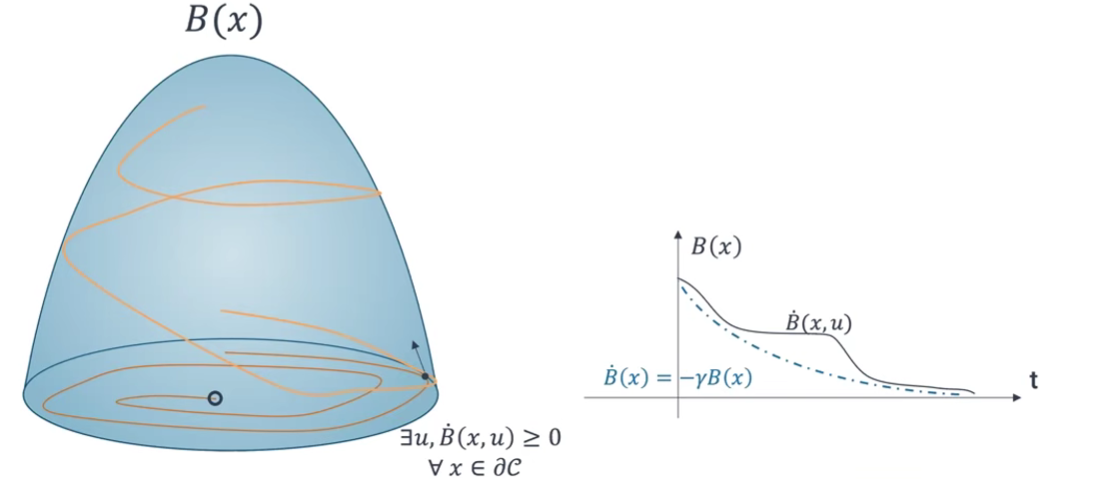
\includegraphics[width=\textwidth]{figures/cbf_geometry.png}
\caption[Barrier geometry and boundary behavior]{Barrier geometry and boundary behavior. The safe region satisfies $B(x)\geq0$. On its boundary, an admissible input must satisfy $\dot B(x,u)\geq0$; inside, a controlled decrease of $B$ is permitted.}
\label{fig:cbfgeometry}
\end{figure}

CBFs are a conceptual dual of the CLFs introduced in Section~\ref{ch:navigation}: a CLF decreases toward a target, whereas a CBF prevents departure from a set. A robot can remain safe without reaching its goal, or converge to a goal along an unsafe route. These objectives are therefore complementary.

For obstacle avoidance, the safe set can encode a required clearance around the robot rather than only the obstacle's visible surface. A configuration outside this region is inadmissible even if no contact has yet occurred. The chosen set should reflect the physical task and the information available to evaluate it.

Forward invariance connects a local condition on the current motion to the preservation of the set over time. The boundary matters because crossing it changes a safe state into an unsafe one. Inside the set, the robot retains freedom to move toward its task objective~\cite{litAmes2019}.

\subsection{The Barrier Condition}
For the nominal dynamics $\dot x=f(x)+g(x)u$, the chain rule gives
\begin{equation}
\dot B(x,u)=L_fB(x)+L_gB(x)u,
\quad L_fB=\nabla B^\top f,\quad L_gB=\nabla B^\top g.
\end{equation}
A continuously differentiable function $B$ is a CBF on a domain containing $\mathcal C$ if an admissible input can satisfy
\begin{equation}
L_fB(x)+L_gB(x)u\geq-\alpha(B(x)),
\label{eq:cbfcondition}
\end{equation}
where $\alpha$ is an extended class-$\mathcal K$ function: it is continuous, strictly increasing, and $\alpha(0)=0$~\cite{litAmes2017}. Unlike requiring $\dot B\geq0$ everywhere, this condition permits motion toward the boundary while limiting the approach rate.

For $\alpha(B)=\kappa B$, $\kappa>0$, direct integration yields
\begin{equation}
\frac{d}{dt}\left(e^{\kappa t}B(x(t))\right)\geq0
\quad\Longrightarrow\quad
B(x(t))\geq e^{-\kappa t}B(x(0))\geq0.
\end{equation}
The bound applies when the inequality holds along the trajectory and $B(x(0))\geq0$. More generally, forward invariance follows under the CBF theorem's regularity assumptions: locally Lipschitz dynamics and enforcing feedback, a regular boundary, and feasible inputs. The guarantee holds over the solution's existence interval; forward completeness extends it to all future time~\cite{litAmes2017}.

The function $\alpha$ determines how the allowed approach rate changes with the barrier value. Far from a constraint, the controller may have considerable freedom; closer to the boundary, the condition limits motion that would consume the remaining margin too quickly. This goes beyond checking whether the current position is collision-free.

Feasibility connects the geometry of the safe set to the available control authority. If the robot cannot brake strongly enough, a formally written inequality may demand an unavailable command. The existence of an admissible input is therefore part of the safety argument.

\subsection{Filtering a Learned Control Input}
Let $u_{\rm RL}$ be the command proposed by the navigation policy. A CBF filter selects a nearby admissible command by solving
\begin{equation}
\begin{aligned}
u^*(x)=\argmin_{u\in\mathcal U}\quad&\frac12\norm{u-u_{\rm RL}}^2\\
\text{subject to}\quad&L_fB(x)+L_gB(x)u\geq-\alpha(B(x)).
\end{aligned}
\label{eq:cbfqp}
\end{equation}
For a closed convex input set and a feasible constraint, this projection preserves an already admissible command and otherwise makes the smallest Euclidean correction. A CLF inequality can be included to encourage convergence, usually with a relaxation variable so that the stability objective can yield to the safety constraint~\cite{litAmes2017}.

The filter's guarantee depends on the model used in its constraint. For the disturbed dynamics of Section~\ref{ch:navigation}, the actual derivative contains the additional term $\nabla B(x)^\top d(t)$. Unknown wind must therefore be estimated or bounded when constructing the safety condition. Likewise, continuous-time enforcement does not follow from checking the inequality only at discrete control updates.

For several obstacles, the filter can include a condition for each relevant boundary. An action that is acceptable with respect to one obstacle may conflict with another, so the constraints must be considered together. An already admissible command is preserved, allowing the task policy to determine ordinary motion while the filter intervenes near active constraints.

The objective measures correction size; the constraints express safety. A nearby command is useful only if it satisfies those constraints.

\clearpage
\subsection{High-Order Control Barrier Functions}
A constraint has relative degree $r$ when the control input first appears in its $r$th time derivative. If $r>1$, the first-order condition cannot directly select $u$. High-order control barrier functions (HOCBFs) address this by recursively defining~\cite{litXiao2019}
\begin{equation}
\psi_0(x)=B(x),\qquad
\psi_i(x)=\dot\psi_{i-1}(x)+\alpha_i(\psi_{i-1}(x)),
\quad i=1,\ldots,r.
\end{equation}
Here the $\alpha_i$ are sufficiently smooth class-$\mathcal K$ functions. The final expression $\psi_r(x,u)$ contains the input. Enforcing $\psi_r\geq0$ preserves the intersection
\begin{equation}
\mathcal C_r=\bigcap_{i=0}^{r-1}\{x:\psi_i(x)\geq0\},
\end{equation}
provided the initial state lies in this intersection, the functions are sufficiently smooth, and a feasible regular feedback enforces the condition. Recursively applying the comparison argument then preserves each $\psi_i\geq0$, including $B\geq0$~\cite{litXiao2019}.

A braking example gives the intuition. Two vehicles can be at the same distance from a wall while having different opportunities to avoid it: one is nearly stationary, while the other approaches rapidly. A position-only snapshot treats their clearance equally, but a higher-order condition also accounts for how that clearance is changing. The controller must act early enough for the dynamics to respond.

\clearpage
For a simple acceleration-controlled navigation model, consider
\begin{equation}
\dot p=v,\qquad\dot v=u,\qquad
B(p)=\norm{p-p_o}^2-R^2,
\end{equation}
where $p_o$ is a fixed obstacle center and $R>0$ is the exclusion radius. Writing $e=p-p_o$ gives
\begin{equation}
\dot B=2e^\top v,\qquad
\ddot B=2\norm{v}^2+2e^\top u.
\end{equation}
The acceleration input appears only in the second derivative. With linear functions $\alpha_i(s)=k_i s$, $k_i>0$, the HOCBF constraint becomes
\begin{equation}
\ddot B+(k_1+k_2)\dot B+k_1k_2B\geq0.
\label{eq:hocbfsecondorder}
\end{equation}
Its initial conditions include both $B\geq0$ and $\dot B+k_1B\geq0$: clearance alone is insufficient when the robot approaches an obstacle too quickly. This explains the relevance to drones and other mechanical systems. The required relative degree depends on the chosen safety function and control interface, rather than the robot's name. Actuator limits can still make the HOCBF constraint infeasible.

\begin{figure}[H]
\centering
\begin{tikzpicture}[x=1cm,y=1cm,>=Stealth,font=\small]
\fill[gray!35] (9,-.45) rectangle (9.55,2.45);
\draw[gray!70,thick] (9,-.45)--(9,2.45);
\node[anchor=south] at (9.25,2.6) {Obstacle};
\draw[dashed,gray!65] (5,-.45)--(5,2.5);
\node[anchor=west] at (0,2) {Slow approach};
\node[anchor=west] at (0,0) {Fast approach};
\fill[teal] (5,2) circle (.13);
\fill[teal] (5,0) circle (.13);
\draw[->,very thick,teal] (5.2,2)--(6.15,2);
\draw[->,very thick,teal] (5.2,0)--(8.15,0);
\draw[<->,black!70] (5,-.85)--node[below]{Same clearance}(9,-.85);
\end{tikzpicture}
\caption[Clearance and approach speed]{Equal geometric clearance can require different braking responses. The arrows represent approach velocity: the faster state needs earlier intervention under limited acceleration.}
\label{fig:hocbfbraking}
\end{figure}

\FloatBarrier
\section{Reinforcement Learning with Control Barrier Functions}
\label{ch:rlcbf}

\subsection{Task Learning with a Safety Layer}
RL and CBFs give complementary responsibilities to an embodied controller. The RL policy chooses actions to accomplish a task, such as following a route or reaching a goal. The CBF layer checks those actions against a safety condition and corrects them when necessary. The policy supplies task-directed behavior; the filter restricts the commands applied to the robot.

For the nominal policy command $u_{\rm RL}$, this architecture is
\begin{equation}
u_{\rm RL}=\pi_\theta(o),\qquad
u_{\rm applied}=\operatorname{CBFfilter}(x,u_{\rm RL}),
\end{equation}
where $o$ is the policy observation and $x$ is the state information used by the filter. Under the assumptions of Section~\ref{ch:cbf}, continuous enforcement of a feasible CBF constraint guarantees forward invariance of the safe set. This provides a formal safety layer around learned decisions. The guarantee requires a valid model, safe initialization, and an implementation that enforces the condition; combining two modules alone is insufficient.

\begin{figure}[htbp]
\centering
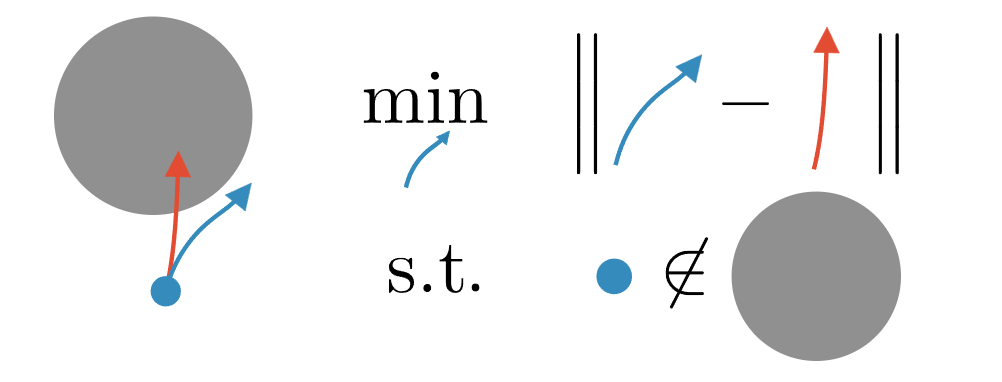
\includegraphics[width=.90\textwidth]{figures/pncbf_filter_concept.png}
\caption[Safety filtering of a nominal action]{Safety filtering of a nominal action. The red command points toward an obstacle; the blue correction preserves safety while remaining close to it. Illustration by So et al., PNCBF project page~\cite{litPNCBFProject}.}
\label{fig:rlcbfconcept}
\end{figure}

This division of responsibilities allows the policy to choose among several ways to accomplish a task while the filter excludes inadmissible commands. A correction is local to the current decision; it does not replace route planning or guarantee that every safe action eventually reaches the goal.

The components also need consistent information. The nominal command must use the same control coordinates as the filter output, and the barrier must be evaluated with an appropriate state estimate. Otherwise, the optimized correction may not correspond to the intended change in physical motion.

\subsection{Learning with CBF Corrections}
CBF-RL integrates the safety mechanism into training~\cite{litCBFRL2026}. Its \emph{Filter Only} variant corrects policy actions before execution. \emph{Reward Only} uses a barrier-inspired reward, while \emph{Dual} combines filtering and reward shaping. The reward encourages the policy to propose actions that need less correction. \emph{Nominal} provides the comparison without these additions.

Applying corrections during training changes the experience collected by the policy. A proposed action can produce a transition governed by the filtered action. CBF-RL combines this intervention with reward shaping so that the policy can learn to propose commands requiring fewer corrections~\cite{litCBFRL2026}.

\begin{figure}[htbp]
\centering
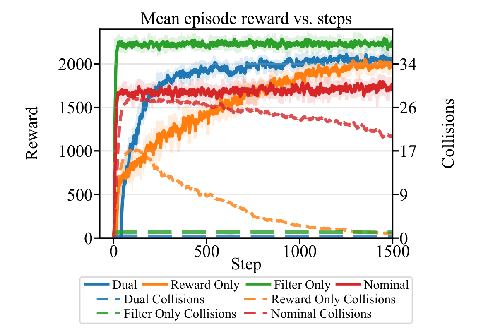
\includegraphics[width=.66\textwidth]{figures/cbfrl_training_original.pdf}
\caption[Training reward and collisions in CBF-RL]{Training reward and collisions in the 2D navigation experiment of Yang et al.~\cite{litCBFRL2026}, Fig.~3. Solid curves show rewards and dashed curves show collisions. These are the authors' experimental results.}
\label{fig:rlcbftraining}
\end{figure}

Figure~\ref{fig:rlcbftraining} shows rapid reward improvement and substantially fewer training collisions with filtering. Filter Only reaches a high reward early, while Dual improves faster than Reward Only over much of training. The horizontal axis measures training steps, not elapsed computation time.

The paper also evaluates deployment without a filter: Filter Only degrades markedly when its filter is removed. Empirical policy safety therefore does not replace the guarantee of an actively enforced CBF~\cite{litCBFRL2026}.

The comparison separates safer exploration from improvements in the policy itself. Fewer training collisions can make data collection more useful, but it remains necessary to identify which mechanism is active during execution. Evaluating a policy with and without its runtime filter reveals how much of the observed behavior depends on that intervention.

\subsection{Barrier Learning with Policy Neural CBFs}
A complementary approach learns the safety function itself. Policy neural CBFs (PNCBFs) approximate a nominal policy's maximum-over-time safety cost from rollouts, then use this value function to support safety filtering~\cite{litPNCBF2023}.

So et al. demonstrate the approach on a 16-dimensional F-16 model and two quadrotors in hardware~\cite{litPNCBF2023}. These examples illustrate the reach of learned safety filters, although approximation accuracy and CBF validity remain necessary for a formal guarantee.

The maximum-over-time cost accounts for unsafe behavior that may occur later in a trajectory. A policy can initially move away from an obstacle and still encounter another constraint farther along its route. Rollouts therefore provide information beyond current geometric clearance.

Learning a barrier is attractive when constructing one by hand is difficult. However, learning a useful representation and verifying its barrier property remain distinct tasks. The neural model approximates the relevant function; the safety argument depends on the conditions satisfied by that approximation~\cite{litPNCBF2023}.

\subsection{Disturbance Randomization and Wind Robustness}
The 2D navigation experiment in CBF-RL randomizes dynamics using additive Gaussian perturbations~\cite{litCBFRL2026}. This does not establish robustness to persistent wind or gusts. Turbulence models introduce temporal structure: Dryden filters shape white noise into correlated gust signals~\cite{litDryden2018}. Gaussianity alone therefore does not describe a disturbance's temporal behavior.

The disturbance time scale matters because feedback needs time to respond. Independent perturbations can partly cancel across successive steps, while a sustained force can displace the vehicle in one direction for longer. Testing across these structures helps distinguish tolerance to isolated deviations from adaptation to a changed operating condition.

For example, two disturbance sequences can have similar distributions of instantaneous values while differing in their ordering. One may change direction frequently, whereas the other may retain a directional bias over several control updates. The resulting motion need not be the same because the vehicle carries velocity and the controller reacts with finite delay. This illustrates why a histogram of disturbance magnitudes is not a complete description of a navigation test.

A useful evaluation therefore considers disturbance strength together with persistence, changes during a mission, and the available obstacle clearance. These choices help identify whether the controller merely tolerates sampled perturbations or responds effectively when conditions shift. The prior work in Section~\ref{ch:disturbanceprior} offers several ways to address that response.

This raises the question: \emph{can such a policy maintain reliable navigation and safety under persistent wind, gusts, and disturbance shifts beyond training conditions?}

\FloatBarrier
\section{Navigation Under Disturbance}
\label{ch:disturbanceprior}

Wind can displace a robot from its planned trajectory even when the nominal navigation policy performs well. Rejecting that disturbance requires the controller to respond to effects that may be uncertain, persistent, or changing during flight. Classical approaches use feedback, estimation, and robust design; learning methods add representations or policies that can adapt from experience. The following works mainly address motion control and trajectory tracking, which support navigation but do not by themselves guarantee obstacle avoidance.

\subsection{Classical Methods}

\FloatBarrier
\subsubsection{\texorpdfstring{$\mathcal L_1$}{L1} Adaptive Control}
The $\mathcal L_1$ architecture of Cao and Hovakimyan combines rapid adaptation with a low-pass filter in the control channel~\cite{litL1Original2006}. A state predictor measures the discrepancy between expected and observed motion. An adaptation law estimates the uncertainty, while the filter limits the frequency content of the resulting control correction. This separates fast estimation from the bandwidth of the commands sent to the actuators.

The original analysis establishes transient tracking bounds for its uncertain linear-system setting under a small-gain condition and bounded-parameter assumptions. In quadrotor control, Hanover et al. combine an $\mathcal L_1$ augmentation with nonlinear MPC to compensate for model mismatch and payload changes~\cite{litHanover2022}. The practical design must balance disturbance rejection against sensor noise, delay, and actuator bandwidth.

The estimate need not identify the physical origin of every mismatch. For navigation, its immediate purpose is to support a suitable correction. This makes the architecture useful when payload changes or external forces alter the response, provided those effects remain compatible with the assumptions of the chosen augmentation.

\FloatBarrier
\subsubsection{Incremental Nonlinear Dynamic Inversion (INDI)}
INDI uses measured acceleration to determine how much the control input should change. Instead of reconstructing every aerodynamic force, it starts from the vehicle's observed response and uses a local control-effectiveness model to compute an input increment. Disturbances are therefore reflected in the measured motion and compensated through feedback.

Smeur et al. develop adaptive INDI for micro-air-vehicle attitude control, then extend it to a cascaded structure for disturbance rejection~\cite{litINDI2016,litINDI2018}. The outer loop turns a desired translational acceleration into thrust and attitude commands; the inner loop controls attitude. This reduces dependence on a detailed aerodynamic model, although it still requires reliable acceleration measurements, control-effectiveness estimates, and careful alignment of filtering and actuator dynamics.

Measurement timing is particularly important in an incremental method. Comparing a recently measured acceleration with an input associated with an earlier actuator response can produce a misleading correction. Synchronizing the relevant signals helps the controller interpret the observed motion consistently~\cite{litINDI2016}.

\FloatBarrier
\subsubsection{Disturbance Observers (DOB) and Exponential Smoothing}
A disturbance observer estimates the difference between a nominal model's predicted response and the measured response. Ohnishi's early servo architecture uses estimated load torque to compensate its effect on motion~\cite{litDOB1987}. More generally, the estimate combines external disturbances and model mismatch into an equivalent disturbance, avoiding separate identification of every aerodynamic contribution.

Filtering is central to this design. Sariyildiz and Ohnishi show that measurement filtering affects the stability and robustness of a DOB and constrains its usable bandwidth~\cite{litDOB2015}. A higher observer bandwidth can track faster disturbances, but also exposes the controller to measurement noise and neglected dynamics.

An exponential moving average (EMA) is a simple first-order smoothing option for a sampled disturbance estimate: each update blends the new estimate with its previous filtered value. Stronger smoothing suppresses rapid fluctuations but delays the response to gusts. EMA is a filtering component, not a complete observer; the model and measurements must first supply an estimate to filter. Its suitability depends on the disturbance time scale and the available feedback rate.

A filtered estimate can therefore remain smooth while temporarily lagging a changing disturbance. Its usefulness should be assessed together with the resulting motion, rather than from smoothness alone. This links observer design to the clearance and recovery time available in the navigation task.

\FloatBarrier
\subsubsection{\texorpdfstring{$H_\infty$}{H-infinity} Robust Control}
$H_\infty$ control approaches disturbance rejection through a worst-case performance criterion. In the formulation of Doyle et al., the external input $w$ includes disturbances and measurement noise, while the regulated output $z$ represents weighted errors and other performance objectives~\cite{litHinf1989}. The controller limits the closed-loop amplification from $w$ to $z$, measured by its induced energy gain. It therefore does not require a specific Gaussian disturbance distribution.

The seminal state-space result constructs controllers for a finite-dimensional linear time-invariant model using algebraic Riccati equations. For flight control, the designer must choose a suitable model and performance weights, balancing tracking accuracy, disturbance attenuation, and control effort. The resulting bound concerns the modeled input-output behavior; it does not establish collision avoidance for an arbitrary nonlinear vehicle under unlimited wind.

The performance weights determine which errors the design prioritizes. For example, reducing position error more aggressively can require greater control effort. Robust synthesis makes that trade-off explicit within the model; the selected weights and available actuators determine whether the resulting design is useful for a particular vehicle.

\subsection{Learning Methods}
Deep learning makes it possible to represent complex dynamics and train controllers across varied operating conditions. The methods below differ in what adapts: an adversarially trained policy, a latent description of the environment, an aerodynamic force model, or the policy parameters.

\FloatBarrier
\subsubsection{Adversarial Reinforcement Learning: REFORMA}
REFORMA trains a drone controller against a group of adversaries that perturb its actions~\cite{litREFORMA2024}. The protagonist learns to complete hovering and traversal tasks while the adversaries seek to reduce its return. Training emphasizes the average performance against the adversaries inducing the lowest protagonist returns, exposing the controller to challenging interactions beyond randomly sampled perturbations.

The adversary strength $\alpha$ controls the mixing of protagonist and adversary actions. A factor encoder forms $z_t$ from environment parameters, states, and protagonist and attacked actions. An adaptation module predicts this representation from recent state/action histories to condition the policy at deployment. Neither module receives $\alpha$ explicitly; disturbance strength is inferred through the observed interaction (Figure~\ref{fig:reforma}).

\begin{figure}[H]
\centering
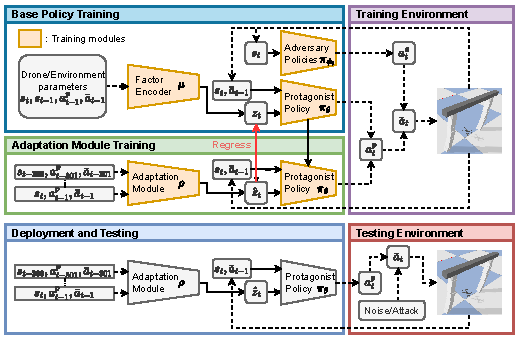
\includegraphics[width=.96\textwidth]{figures/reforma_architecture.pdf}
\caption[REFORMA training and adaptation]{REFORMA: adversarial policy training, adaptation-module training, and deployment. From Hsu et al.~\cite{litREFORMA2024}, Fig.~1. Symbols retain the authors' notation.}
\label{fig:reforma}
\end{figure}

The authors evaluate the method in simulation. Their results support robustness to the tested action disturbances, but the adversary's action space and strength still define which challenges training can represent. Adversarial training does not automatically cover every physical wind field.

Using several adversaries broadens the challenging interactions encountered during training. However, they still act through the disturbance mechanism defined by the environment. This makes the design of the adversary meaningful: robustness to an action perturbation should be interpreted in relation to the physical effect that perturbation is intended to represent.

\FloatBarrier
\subsubsection{Rapid Motor Adaptation (RMA)}
Rapid Motor Adaptation separates a base policy from a module that infers the current operating conditions~\cite{litRMA2021}. Kumar et al. introduce this architecture for quadruped locomotion at RSS 2021. Its relevance to flight is the general adaptation principle: recent motion contains information about dynamics that are not directly measured.

\begin{figure}[H]
\centering
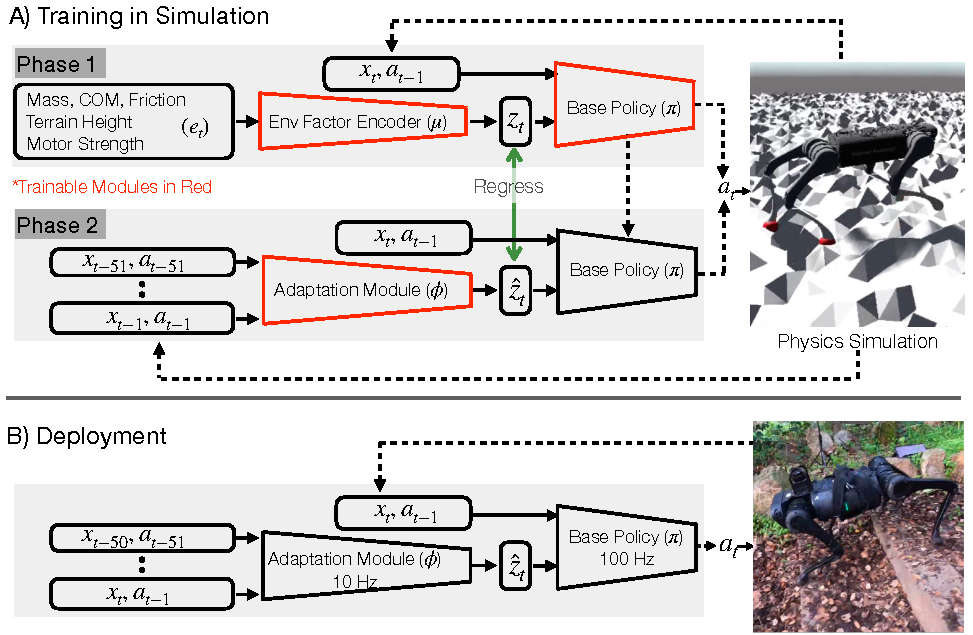
\includegraphics[width=\textwidth]{figures/rma_architecture.pdf}
\caption[Rapid Motor Adaptation architecture]{RMA's two training phases and deployment architecture. From Kumar et al.~\cite{litRMA2021}, Fig.~2. The adaptation module estimates the latent operating conditions used by the base policy.}
\label{fig:rma}
\end{figure}

\Needspace{3\baselineskip}
During simulation training, an encoder $\mu$ converts privileged environmental factors $e_t$, such as friction and payload, into a latent vector $z_t$. The policy $\pi$ uses this vector alongside the robot state and previous action. A second training phase teaches an adaptation module $\phi$ to estimate $\hat z_t$ from a history of states and actions. Deployment uses this estimate instead of privileged simulator information.



RMA adapts its latent input online without retraining the policy weights on the robot. The authors demonstrate locomotion over varied real terrain and changing conditions. These experiments establish a useful precedent for adaptation from motion history, while their legged-robot results are not a direct evaluation of aerial wind rejection.

The latent vector need not recover each physical parameter separately. It needs to retain information that helps the policy select an appropriate response. This reduces the burden of explicit identification, although ambiguous or unfamiliar motion histories can still make adaptation difficult~\cite{litRMA2021}.

\FloatBarrier
\subsubsection{Neural-Fly: Learned Aerodynamics with Adaptive Control}
Neural-Fly combines a learned aerodynamic representation with a structured online adaptation law~\cite{litNeuralFly2022}. O'Connell et al. train a neural basis using flight data from different wind conditions. Their domain-adversarially invariant meta-learning procedure seeks a shared representation whose coefficients can change with the wind.

Using the authors' notation, the force estimate has the form $\hat f=\phi\hat a$: the learned basis $\phi$ is fixed during deployment, while the coefficients $\hat a$ adapt online. The update uses both tracking error and force-prediction error. This retains a conventional feedback controller and concentrates online learning in a compact set of parameters.

\begin{figure}[H]
\centering
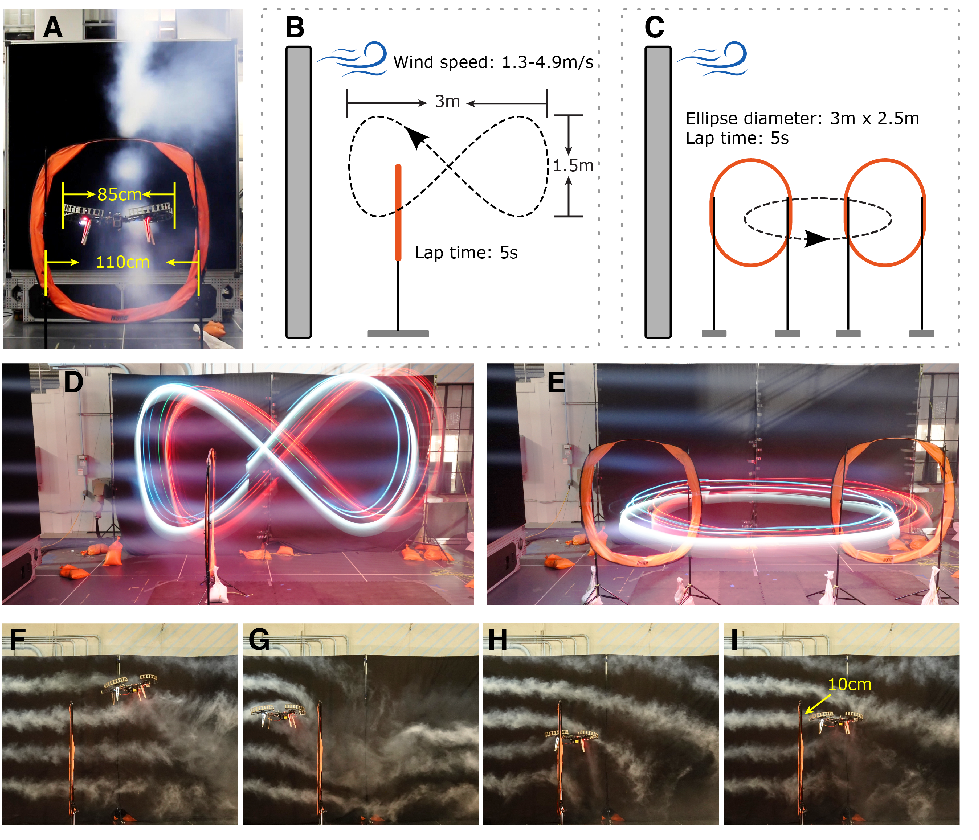
\includegraphics[width=.86\textwidth]{figures/neuralfly_flight.pdf}
\caption[Neural-Fly flight experiments]{Wind-tunnel setup, reference trajectories, and gate-passing photographs from O'Connell et al.~\cite{litNeuralFly2022}, Fig.~1. These panels illustrate the authors' physical flight experiments.}
\label{fig:neuralfly}
\end{figure}

The Science Robotics study reports experiments in winds up to $12.1\,\mathrm{m\,s^{-1}}$ and improved tracking over its comparison controllers. Its gate experiments illustrate precise flight under wind, while its stability analysis bounds the effect of imperfect learning under stated assumptions. Neural-Fly is a learning-based adaptive controller; its domain-adversarial representation learning is distinct from REFORMA's adversarial RL action perturbations.

The compact online update is a central design choice. The learned basis captures reusable aerodynamic structure, while the changing coefficients respond to the current conditions. This gives the adaptive part a clear role inside the feedback loop without retraining the entire representation during each flight~\cite{litNeuralFly2022}.

\FloatBarrier
\subsubsection{DATT: Deep Adaptive Trajectory Tracking}
DATT combines feedforward trajectory information, state feedback, and disturbance adaptation in an RL policy~\cite{litDATT2023}. A learned encoder summarizes upcoming reference positions, allowing the policy to anticipate turns. State feedback describes the current motion, while a disturbance input tells the controller how the observed dynamics differ from the nominal model.

\begin{figure}[H]
\centering
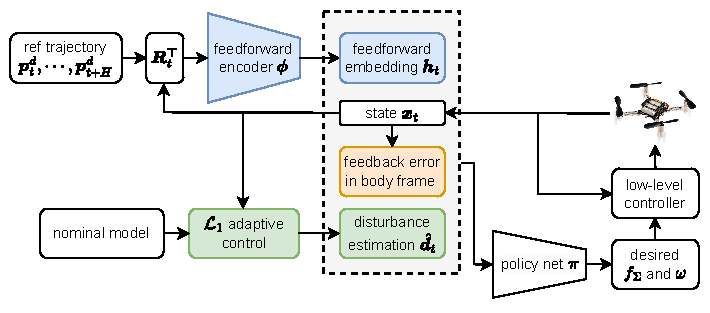
\includegraphics[width=\textwidth]{figures/datt_architecture.pdf}
\caption[DATT feedforward, feedback, and adaptation]{DATT architecture from Huang et al.~\cite{litDATT2023}, Fig.~2. Blue, yellow, and green identify feedforward, feedback, and adaptation components. The authors distinguish the simulated disturbance $d$ from its runtime estimate $\hat d$.}
\label{fig:datt}
\end{figure}

The policy is trained with PPO in simulation and deployed with an $\mathcal L_1$ disturbance estimator, without policy fine-tuning on hardware. It outputs collective thrust and desired body rates. Experiments include smooth references, sharp-turning trajectories that cannot be followed exactly, and unsteady wind. The objective is to reduce tracking error within the vehicle's capabilities, not to make an infeasible reference physically feasible.

DATT already introduces temporal structure into training disturbances: its disturbance follows a Brownian random walk with Gaussian increments. This is an important distinction from independent additive samples. Consequently, temporally correlated disturbance training is established prior work. The remaining question concerns how well adaptation and safety mechanisms handle disturbance conditions beyond those represented during training.

Looking ahead along the reference helps the controller prepare for a turn before the tracking error becomes large. The disturbance estimate supplies different information: how current motion departs from the nominal response. DATT brings these anticipatory and reactive signals together in the same policy.

\FloatBarrier
\subsubsection{Learning on the Fly: Residual Models and Policy Adaptation}
Learning on the Fly (LoTF) updates a deployed policy through a differentiable simulator~\cite{litLoTF2026}. Pan et al. start with an analytical dynamics model and learn a residual model from recent flight data. Together they form a hybrid simulator that better matches the current vehicle and environment. Gradients through simulated rollouts then update the task policy.



The paper compares full policy adaptation with low-rank adaptation (LoRA). Full adaptation updates all policy parameters. LoRA freezes the pretrained parameters and learns an additive low-rank module, reducing the number of trainable parameters. Here, residual learning corrects the dynamics model; it should not be confused with simply adding a residual action to the controller output.

The authors demonstrate adaptation in simulation and physical flight under disturbances and model mismatch. Unlike RMA, LoTF changes policy parameters during deployment; unlike Neural-Fly, adaptation extends beyond force-estimation coefficients. Its performance depends on the quality of the updated simulator and the policy updates it produces.

\begin{figure}[H]
\centering
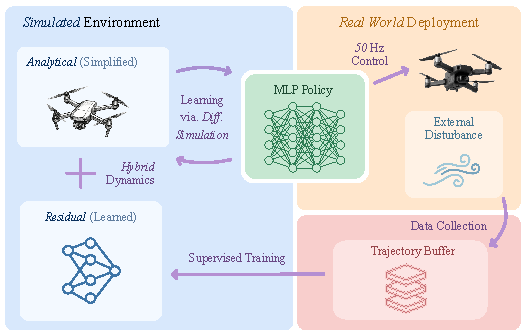
\includegraphics[width=.96\textwidth]{figures/lotf_architecture.pdf}
\caption[Learning on the Fly adaptation loop]{LoTF combines flight-data collection, residual dynamics learning, and policy adaptation through differentiable simulation. From Pan et al.~\cite{litLoTF2026}, Fig.~1. The diagram shows the authors' method.}
\label{fig:lotf}
\end{figure}

The rolling flight-data buffer creates a practical adaptation trade-off. Recent samples describe current conditions, while a broader history can stabilize model fitting. The learned model must remain useful for policy optimization as new data arrive; merely fitting the recent measurements is not the whole control objective.

These methods demonstrate several routes to adaptation, with different requirements for models, representative data and online updates. For a connected robot, a complementary objective is to make recent motion directly useful to a compact safety layer. Chapter~\ref{ch:contribution} develops this idea through disturbance estimation and residual uncertainty, using a rolling window of prediction errors to update the CBF safety margin.

\chapter{System Model and Problem Formulation}
\label{ch:system}

\section{Navigation Task and Control Architecture}
The navigation task is to reach a goal or follow a reference route while avoiding obstacles under unknown disturbances. The reinforcement-learning policy proposes a nominal command, and a control barrier function filter adjusts that command before it is applied. A low-level controller realizes the requested motion. The policy is trained in advance and remains fixed during the evaluation; disturbance estimation and safety-margin adaptation operate online.

The control-affine and disturbed dynamics introduced in Section~\ref{ch:navigation} provide the general background. Here, the model is specified at the velocity-command interface used by the proposed safety layer.

\section{Velocity-Command Model and Disturbance}
We express the filter at the velocity-command interface. Let $p\in\R^3$ be position, $u_B$ the yaw-aligned body-frame command and $R$ the known rotation into world coordinates:
\begin{equation}
 \dot p=Ru_B+d,\qquad
 \mathcal U_B=[-u_{\max},u_{\max}]^3.
 \label{eq:contribution_model}
\end{equation}
The effective disturbance $d$ represents the motion mismatch at this interface, including the effect of wind on velocity tracking. The low-level controller realizes the requested motion.

\section{Clearance Barrier and Safety Constraint}
For a differentiable clearance barrier $B(p)$ with nonzero gradient, write
\begin{equation}
 a=\nabla B(p),\qquad a_B=R^\top a,\qquad
 n=\frac{a}{\norm{a}_2}.
 \label{eq:contribution_normal}
\end{equation}
The unit normal $n$ points toward increasing clearance. The corresponding CBF condition is $a_B^\top u_B+a^\top d+\alpha B(p)\geq0$, with $\alpha>0$. Keeping the command in its original body frame preserves the componentwise input bounds.

\section{Problem Formulation}
The problem is to select an admissible executed command that stays close to the policy proposal while accounting for clearance loss caused by the unknown disturbance. The available information consists of measured motion, the previously executed command, the current clearance barrier and the known body-to-world rotation. Recent motion mismatch supplies the disturbance estimate and residual history.

A fixed margin cannot respond to changing disturbance conditions. The proposed solution therefore constructs an online allowance from the estimated disturbance and the adverse tail of recent residuals, then incorporates it into the bounded CBF projection. Chapter~\ref{ch:contribution} gives this construction and its optimization problem. The safety interpretation retains the model, feasibility and enforcement requirements discussed in Section~\ref{ch:cbf}.

\section{Evaluation Settings}
The static benchmark compares deployed safety filters using known obstacle geometry and a frozen policy. The Isaac Sim and MuJoCo extension adds richer physics and local perception. Section~\ref{sec:simulation_setup} introduces both environments before the results, including the static-arena dimensions, obstacle configurations and evaluation conventions.

\chapter{Adaptive Barrier Filtering for Disturbance-Aware Navigation}
\label{ch:contribution}
\section{Adaptive Safety Layer for the Navigation Policy}

The RL policy proposes a nominal action, and the CBF layer filters it before execution. This follows the division between task learning and safety filtering introduced in Section~\ref{ch:rlcbf} and in CBF-RL~\cite{litCBFRL2026}. In our construction, the observer and residual window update during deployment; the policy weights remain unchanged.

\begin{figure}[H]
\centering
\begin{tikzpicture}[font=\small,>=Latex,
 block/.style={draw=navy,rounded corners=3pt,fill=lightblue!55,align=center,minimum height=1.4cm,text width=3.3cm,inner sep=5pt},
 update/.style={block,draw=teal,fill=teal!8},
 flow/.style={->,thick,draw=navy}]
\node[block] (policy) at (0,0) {RL policy\\\footnotesize fixed parameters};
\node[block] (filter) at (4.8,0) {CBF filter\\\footnotesize bounded projection};
\node[block] (robot) at (9.6,0) {Robot\\\footnotesize executed motion};
\node[update] (observer) at (9.6,-3.1) {Disturbance\\observer\\\footnotesize estimate and residual};
\node[update] (risk) at (4.8,-3.1) {Wasserstein--CVaR\\\footnotesize residual buffer and margin};
\draw[flow] (policy) -- node[above] {$u_{B,\mathrm{nom}}$} (filter);
\draw[flow] (filter) -- node[above] {$u_B^\star$} (robot);
\draw[flow] (robot) -- node[right,align=left,font=\footnotesize] {motion and\\last command} (observer);
\draw[flow,teal] (observer) -- (risk);
\draw[flow,teal] (risk) -- node[right,font=\footnotesize] {margin $m_k$} (filter);
\end{tikzpicture}
\caption[Online disturbance adaptation around a frozen policy]{Proposed information flow. Each observer update uses a completed motion interval and its executed command. The estimate and residual history determine the margin $m_k$, while the navigation policy remains fixed.}
\label{fig:contribution_architecture}
\end{figure}

The velocity-command model, clearance normal and CBF condition are defined in Chapter~\ref{ch:system} (Equations~\eqref{eq:contribution_model} and~\eqref{eq:contribution_normal}).

\section{EMA Estimation and Rolling Residual Window}

\subsection{Disturbance Estimate Update}

At update $k$, the completed motion interval provides a displacement and its previously executed world-frame command $u^\star_{W,k-1}$. With sampling interval $\Delta t$, the observer computes
\begin{align}
 d^{\mathrm{raw}}_{k-1}
 &=\frac{p_k-p_{k-1}}{\Delta t}-u^\star_{W,k-1},
 \label{eq:contribution_raw}\\
 r_{k-1}&=d^{\mathrm{raw}}_{k-1}-\hat d_{k-1},
 \label{eq:contribution_residual}\\
 \hat d_k&=\hat d_{k-1}+\ell r_{k-1},\qquad 0<\ell<1.
 \label{eq:contribution_observer}
\end{align}
This EMA-inspired observer tracks recent disturbance while smoothing the raw measurements. It uses the disturbance-estimation principle discussed in Section~\ref{ch:disturbanceprior}~\cite{litDOB1987,litDOB2015}. A larger gain follows changes more quickly; a smaller gain produces a smoother estimate.

Reconstruction uses the action actually executed after filtering, so the filter's correction is not mistaken for an external disturbance. The residual is computed against the previous estimate, before the EMA update. It therefore records the prediction error present during that completed interval.

The raw quantity is an interval-average motion mismatch. Position noise and imperfect command tracking can contribute to it alongside wind. We use the residuals of this observable mismatch directly, without fitting a separate aerodynamic model.

\subsection{Recent Prediction Error Window}

The rolling window keeps at most $M$ residual vectors. For $k\geq1$, its index set and empirical distribution are
\begin{equation}
\begin{aligned}
 \mathcal I_k&=\{\max(0,k-M),\ldots,k-1\},\qquad N_k=|\mathcal I_k|,\\
 \widehat P_k&=\frac1{N_k}\sum_{i\in\mathcal I_k}\delta_{r_i}.
\end{aligned}
\label{eq:contribution_empirical}
\end{equation}
Once the window is full, each new residual replaces the oldest one. The empirical distribution therefore moves with the recent operating conditions instead of retaining the entire mission history.

A shorter window emphasizes responsiveness; a longer window retains more information about infrequent errors. The window has a fixed capacity but advances in time. It is this renewal of its contents that supplies the online adaptation.

No Gaussian density or mixture model is fitted. The sample cloud can be asymmetric or multimodal, and the original residual vectors remain available for projection onto the current obstacle direction. This makes the temporal observations directly usable by the safety layer.

\section{Wasserstein Neighborhood of the Residual Distribution}

\subsection{Transport Distance}

A new residual need not coincide with any point in the current empirical distribution. Wasserstein distance gives a geometric meaning to this displacement. For distributions with finite first moments, the 1-Wasserstein distance with Euclidean ground cost is
\begin{equation}
 W_1(P,Q)=\inf_{\Gamma\in\Pi(P,Q)}
       \int\norm{r-s}_2\,d\Gamma(r,s),
 \label{eq:contribution_wasserstein}
\end{equation}
where $\Pi(P,Q)$ contains the couplings with marginals $P$ and $Q$. It measures the least average distance needed to transport one probability distribution into the other.

The support-based examples in the Wasserstein GAN paper provide useful intuition~\cite{thArjovsky2017}: a distribution can move a small distance without overlapping its original support. Wasserstein distance reflects that movement. In contrast, $D_{\mathrm{KL}}(P\Vert Q)$ is infinite whenever $P$ gives positive probability to a set assigned zero probability by $Q$.

\begin{figure}[htbp]
\centering
\begin{tikzpicture}[font=\small,>=Latex]
\draw[->,navy] (-.5,0) -- (10.5,0) node[right] {$r$};
\foreach \x in {1,4,7}{
 \draw[navy,very thick] (\x,0) -- (\x,1.05);
 \fill[navy] (\x,1.05) circle (3pt);
 \draw[teal,very thick] (\x+1,0) -- (\x+1,1.85);
 \fill[teal] (\x+1,1.85) circle (3pt);
 \draw[->,thick,orange!80!black] (\x,2.35) -- (\x+1,2.35);
}
\node[anchor=west,navy] at (0,3.2) {Empirical masses};
\node[anchor=west,teal] at (5.6,3.2) {Shifted masses};
\node[align=center] at (4.5,-.8) {Same weights, disjoint locations, displacement $\Delta\ne0$};
\node[align=center,fill=lightblue!50,rounded corners,inner sep=8pt] at (4.5,-1.75)
 {$D_{\mathrm{KL}}(P\Vert Q)=\infty$
 \qquad $W_1(P,Q)=|\Delta|$};
\end{tikzpicture}
\caption[Transport distance for displaced empirical samples]{A one-dimensional illustration of the support issue. Three equally weighted point masses are translated by the same nonzero displacement to disjoint locations. Vertical offsets distinguish the two sets; they do not represent different probability weights. Wasserstein distance records the displacement, while KL divergence is infinite. The example follows the support-based intuition of Arjovsky et al.~\cite{thArjovsky2017}.}
\label{fig:contribution_support}
\end{figure}

\FloatBarrier
\subsection{Uncertainty in the Observed Distribution}

For our residual window, construct
\begin{equation}
 \mathcal P_k(\rho)=
 \{Q\in\mathcal P_1(\R^3):W_1(Q,\widehat P_k)\leq\rho\},
 \label{eq:contribution_ball}
\end{equation}
where $\mathcal P_1$ denotes distributions with finite first moments. We write the radius as $\rho$, distinguishing it from the residual vectors $r_i$. The center $\widehat P_k$ changes with the window; the radius sets the allowed disagreement with the observed residual distribution.

\begin{figure}[htbp]
\centering
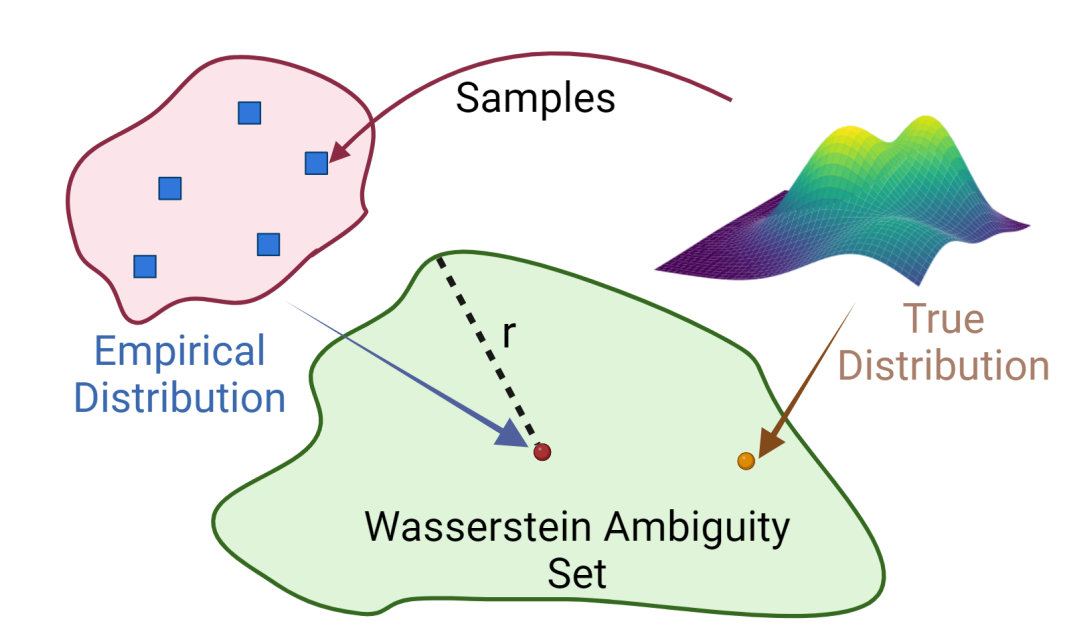
\includegraphics[width=.97\textwidth]{figures/long_wasserstein_ambiguity.png}
\caption[Wasserstein ambiguity set]{Wasserstein ambiguity set, from Long et al.~\cite{long2024sensor}, Fig.~3. The radius labeled $r$ corresponds to $\rho$ here. Each point in the lower schematic represents a distribution, not a residual sample. The true distribution is shown inside the neighborhood as an illustration of the intended coverage.}
\label{fig:contribution_ball}
\end{figure}

This construction admits previously unseen residual values without choosing a parametric density. It also connects to tractable CVaR bounds for affine directional losses~\cite{thEsfahani2018,long2024sensor}. The distributional allowance can consequently be evaluated before the final command projection.

\FloatBarrier
\section{Residual-Based Safety Margin}

\subsection{Adverse Tail of the Residuals}

At the current update, the clearance-reducing residual is $z_k(r)=-n_k^\top r$. Positive values describe unmodeled motion toward the obstacle. Every vector in the window is projected onto the current normal, so the risk calculation follows the present geometry.

Conditional value-at-risk (CVaR) summarizes the adverse tail of these projected residuals. With upper-tail probability $\epsilon\in(0,1)$, the empirical calculation is
\begin{equation}
 \widehat{\cvar}_{\epsilon,k}(z_k)=
 \min_{\eta\in\R}\left\{
 \eta+\frac1{\epsilon N_k}
 \sum_{i\in\mathcal I_k}(z_k(r_i)-\eta)_+
 \right\}.
 \label{eq:contribution_cvar}
\end{equation}
The threshold $\eta$ separates the adverse tail. The positive-part term measures exceedances above it. This definition applies directly to empirical samples, including repeated values and fractional sample mass at the threshold~\cite{thRockafellar2002}.

\begin{figure}[htbp]
\centering
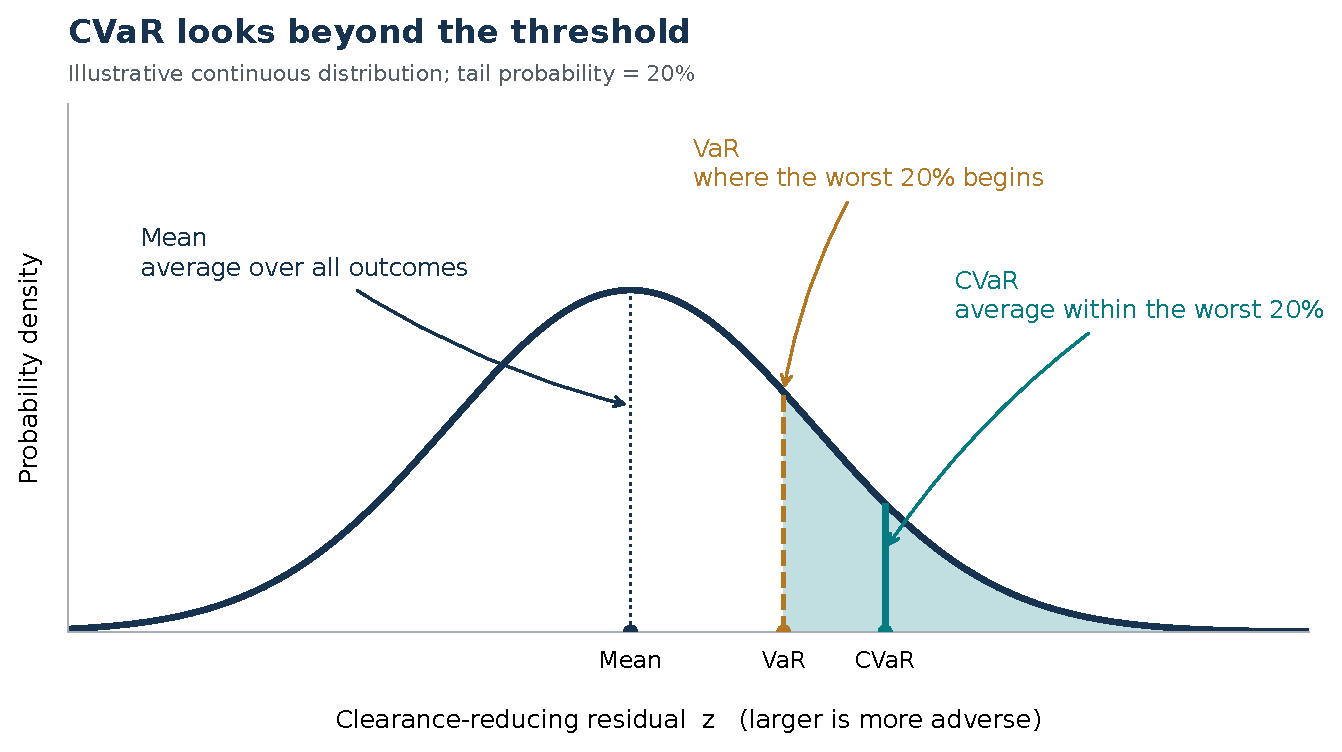
\includegraphics[width=\textwidth]{figures/cvar_tail_explanation.pdf}
\caption[Understanding CVaR through the adverse tail]{The mean averages all outcomes. VaR locates the beginning of the adverse tail; CVaR measures the average loss within that tail for this continuous illustration. The shaded region contains the worst 20\% of outcomes, chosen only to make the concept visible. The density is an explanatory example, not a fitted residual model or experimental result. For an empirical distribution, Equation~\eqref{eq:contribution_cvar} handles the possible fractional mass at the threshold~\cite{thRockafellar2002}.}
\label{fig:contribution_tail}
\end{figure}

\FloatBarrier
\subsection{Estimation and Distributional Uncertainty}

The observer contributes the estimated adverse component $-n_k^\top\hat d_k$. CVaR describes the remaining directional error. For the unit normal and Euclidean transport cost used here, the Wasserstein bound adds the scalar allowance $\rho/\epsilon$~\cite{thEsfahani2018,long2024sensor}. We therefore use
\begin{equation}
 m_k=\left[
 -n_k^\top\hat d_k+
 \widehat{\cvar}_{\epsilon,k}(z_k)+\frac{\rho}{\epsilon}
 \right]_+.
 \label{eq:contribution_margin}
\end{equation}
The three terms account for the estimated disturbance, its observed residual tail and disagreement with the empirical distribution. The positive part keeps the margin nonnegative. W-CVaR adjusts this safety allowance; the EMA observer itself retains its simple update.

The radius and tail probability control the distributional allowance, while the empirical term changes with the window. As large residuals leave the window, the margin can decrease; new adverse errors can increase it. This is intended to avoid maintaining a large constant disturbance allowance when recent conditions no longer call for it.

\section{CBF Filtering with an Adaptive Margin}

The RL policy proposes $u_{B,\mathrm{nom}}$. The safety layer incorporates the updated margin through
\begin{equation}
\begin{aligned}
 u_B^\star={}&\argmin_{v\in\mathcal U_B}
              \frac12\norm{v-u_{B,\mathrm{nom}}}_2^2,\\
 &\text{subject to}\quad
 a_B^\top v\geq-\alpha B(p)+\norm{a}_2m_k.
\end{aligned}
\label{eq:contribution_projection}
\end{equation}
The objective keeps the executed command close to the policy proposal. A nominal action that already meets the adjusted condition passes through unchanged. Otherwise, the projection seeks the smallest correction within the command bounds.

The residual samples enter this optimization through the scalar margin $m_k$. Updating the observer, renewing the window and evaluating its directional tail occur before the three-dimensional command projection. This organization gives online adaptation a compact role inside the RL--CBF loop, without retraining the policy or fitting a residual dynamics network.

After execution, the new motion interval supplies the next residual and the cycle repeats. The design aims to balance responsiveness to disturbance with limited intervention in the learned navigation behavior.

\chapter{Results and Discussion}
\label{chap:results}

\section{Simulation Environment and Setup}
\label{sec:simulation_setup}
\subsection{Static Known-Geometry Benchmark}
The benchmark contains 100 static environments: 60 for training, 20 for validation and 20 for testing. Arenas measure $10\times10\times6.5$\,m, with obstacle occupancy from 1\% to 12.5\% and geometry known to every method. Each start--goal pair has a verified three-dimensional A* reference and a budget based on twice its length.

Commands are issued at 20\,Hz, with each velocity component bounded by 1.5\,m/s. The nominal barrier uses $\alpha=4$ and a 0.28\,m offset: a 0.18\,m vehicle envelope plus a 0.10\,m clearance buffer. An episode succeeds on reaching the 0.40\,m goal region. Its collision event is an overlap of the 0.18\,m evaluation envelope with an obstacle or wall; the collision check takes precedence over goal attainment.

\subsection{Physics-Based Navigation Extension}
The practical extension uses Isaac Sim and MuJoCo, with pillar obstacles and local mapping from simulated LiDAR observations containing noise and missing returns. A planned A* route is smoothed with a B-spline. The three comparison scenarios contain 72 static obstacles together with 12, 20 or 40 dynamic obstacles. The scene views and the NavRL comparison appear in Section~\ref{chap:sim2real}; they complement the known-geometry disturbance benchmark.

\clearpage
\section{Performance Metrics}
\label{sec:performance_metrics}

\subsection{Safety and Episode Outcomes}

We evaluate safe mission completion and tracking accuracy under disturbance using the following performance metrics.

Consider $N$ evaluation episodes. We assign each episode one terminal outcome: success, collision or timeout. Success means reaching the goal within the prescribed tolerance and time limit without collision. A collision ends the episode; an episode that reaches neither a successful goal nor a collision before the time limit is a timeout. If goal attainment and collision occur at the same step, collision takes precedence.

Let $N_{\mathrm{S}}$, $N_{\mathrm{C}}$ and $N_{\mathrm{T}}$ denote the corresponding counts. The success rate (SR), collision rate (CR) and timeout rate (TR) are
\begin{equation}
 \mathrm{SR}=\frac{N_{\mathrm{S}}}{N},\qquad
 \mathrm{CR}=\frac{N_{\mathrm{C}}}{N},\qquad
 \mathrm{TR}=\frac{N_{\mathrm{T}}}{N}.
 \label{eq:episode_rates}
\end{equation}
These fractions are reported as percentages. Under this three-outcome convention, $\mathrm{SR}+\mathrm{CR}+\mathrm{TR}=1$.

\begin{table}[H]
\centering
\caption{Interpretation of the episode-outcome metrics.}
\label{tab:episode_metrics}
\renewcommand{\arraystretch}{1.35}
\begin{tabularx}{\linewidth}{@{}lYc@{}}
\toprule
\textbf{Metric} & \textbf{What it measures} & \textbf{Desired}\\
\midrule
\textcolor{teal}{\textbf{SR}} & Safe mission completion & Higher\\
\textcolor{navy}{\textbf{CR}} & Episodes ending in collision & Lower\\
\textbf{TR} & Episodes exhausting their time budget & Lower\\
\bottomrule
\end{tabularx}
\end{table}

SR measures safe mission completion, CR isolates collision failures, and TR records failure to finish on time. Reading all three together avoids rewarding a controller simply for remaining stationary. Every rate uses the full set of episodes.

\clearpage
\subsection{Tracking Accuracy Under Disturbance}
\label{sec:tracking_accuracy}

Following DATT~\cite{litDATT2023}, let $\bm p_t\in\mathbb R^3$ be the robot position and $\bm p_t^d$ the desired position at discrete time step $t$. For an episode with $T$ evaluated samples, the average tracking error is
\begin{equation}
 E_{\mathrm{track}}=\frac{1}{T}\sum_{t=1}^{T}
 \left\lVert\bm p_t-\bm p_t^d\right\rVert_2.
 \label{eq:average_tracking_error}
\end{equation}
It is expressed in meters. The positions are compared at the same time step, so the metric captures both spatial deviation and delay along the reference. DATT does not require a smooth desired trajectory for this definition; smoothness is a choice in our reference construction.

\medskip
\noindent\textbf{From planned waypoints to a smooth reference.}

We construct the reference from a kinodynamic A* path using a B-spline. A B-spline blends short polynomial pieces into a smooth curve, shaped by nearby control points~\cite{evalDeBoor2001}. This rounds abrupt changes in direction rather than asking the drone to follow a sequence of sharp corners. Control points shape the curve; they need not all lie on it. After smoothing, the path must retain obstacle clearance and respect the motion limits used to assign its timing.

\begin{figure}[H]
\centering
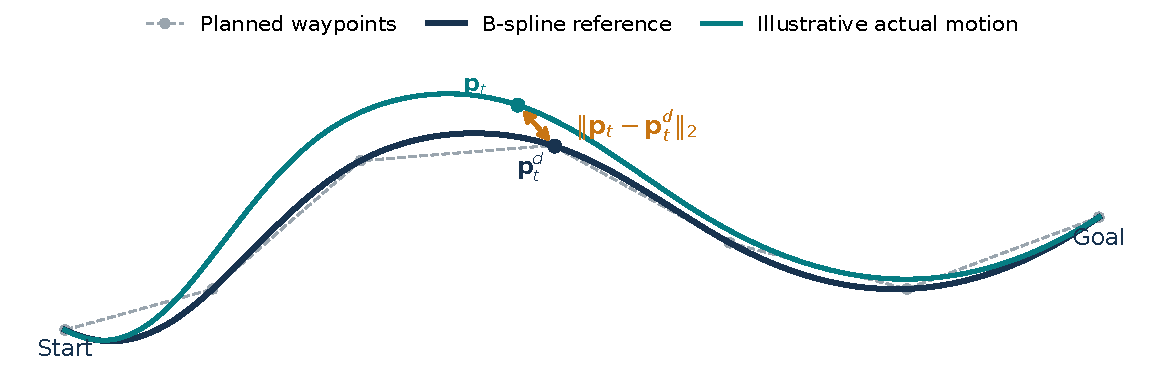
\includegraphics[width=\linewidth]{figures/evaluation_tracking_reference.pdf}
\caption[Smoothed reference and time-matched tracking error]{Conceptual planar view of a three-dimensional tracking task. A B-spline is fitted to planned waypoints; reference samples and actual positions are paired at the same instant. The highlighted separation contributes one term to Equation~\eqref{eq:average_tracking_error}.}
\label{fig:evaluation_tracking}
\end{figure}

A prescribed timing law provides $\bm p_1^d,\ldots,\bm p_T^d$ at the evaluation sampling interval. The reference and its timing are held constant across compared methods.


\clearpage
\section{Curriculum Training}
\label{sec:curriculum_training}

The navigation policy follows a curriculum, progressing from easier tasks toward harder navigation conditions. This lets the policy acquire basic goal-directed behavior before confronting more demanding situations.

The policy has two hidden layers of 64 units. PPO training uses approximately $10^8$ transitions in 4096 parallel environments on an NVIDIA A100, with learning rate $3\times10^{-4}$, discount factor $0.99$ and clipping ratio $0.2$. The environment executes the CBF-corrected command during filtered training, while PPO retains the sampled nominal action.

\begin{figure}[H]
\centering
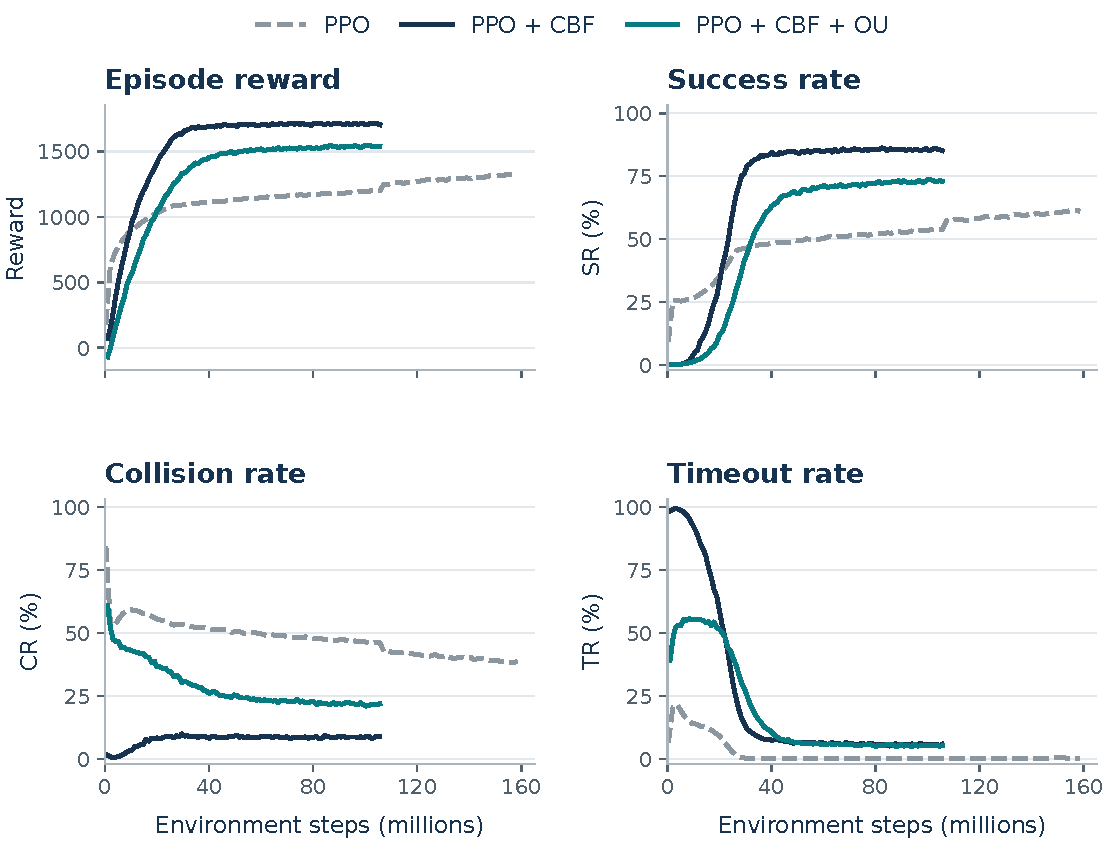
\includegraphics[width=\linewidth]{figures/results_training_curves.pdf}
\caption[Training reward and episode outcomes]{Training reward and episode outcomes for unfiltered PPO, PPO with a CBF filter, and filtered PPO with OU wind. The original plotted values and training horizons are retained. These supplied training histories have no uncertainty bands.}
\label{fig:results_training}
\end{figure}

The no-wind filtered configuration reaches high reward and success earlier in these histories. With OU wind, success rises more gradually and remains lower. The evaluation below holds one policy fixed and changes only the deployed safety filter.

\clearpage
\section{Wind Disturbance Profiles}

Wind is represented through its effect on translational motion. OU profiles retain temporal correlation: successive disturbances fluctuate around a prescribed mean instead of being independent perturbations. The representative profiles in Figure~\ref{fig:results_wind} distinguish drift, stronger sustained disturbance and greater volatility, together with the supplied gust and sinusoidal traces.

\begin{figure}[H]
\centering
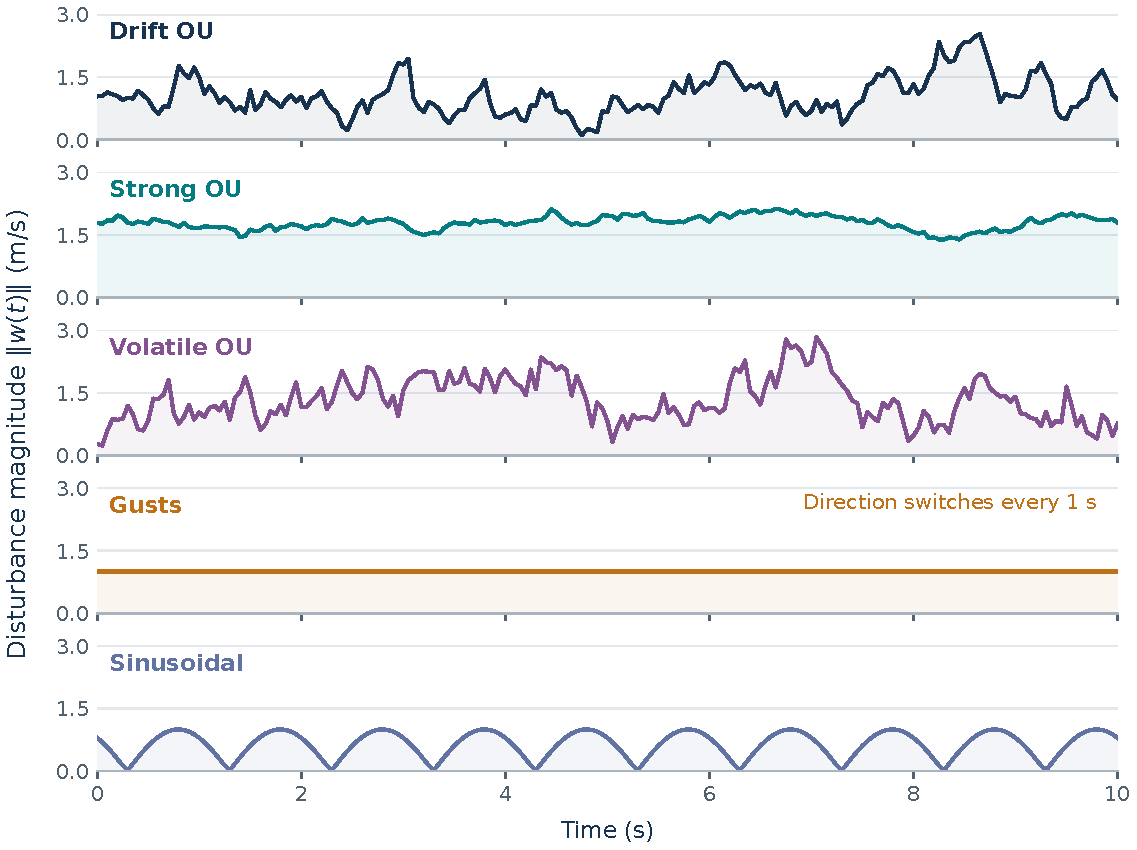
\includegraphics[width=\linewidth]{figures/results_wind_profiles.pdf}
\caption[Representative wind profiles]{Representative disturbance traces with a common magnitude scale. OU denotes Ornstein--Uhlenbeck. The gust profile changes direction every second while retaining a magnitude of 1\,m/s. These are illustrative profiles, not atmospheric measurements.}
\label{fig:results_wind}
\end{figure}

The paired evaluation uses four condition groups: \textbf{calm}, \textbf{steady crosswind}, \textbf{reversing wind} and \textbf{gust-like wind}. Each mission includes one calm condition and five seeded sequences from each noncalm family. These 16 conditions are identical across the compared filters. The five profiles above illustrate temporal behavior; the four benchmark groups define the evaluation split.

\clearpage
\section{Evaluation Protocol}

\subsection{Compared Safety Filters}

All five filters use the same frozen policy: nominal CBF has no disturbance margin; fixed-margin CBF adds 0.50\,m/s; $\mathcal L_1$-style CBF uses disturbance prediction; empirical CVaR-CBF adds the residual tail; and Ours includes the Wasserstein allowance.

For Ours, the observer gain is $0.30I_3$, the residual window contains 64 samples, the tail probability is $\epsilon=0.05$, and $\rho=0.01$\,m/s. The window spans 3.2\,s at the control rate, and the distributional allowance is $\rho/\epsilon=0.20$\,m/s. These settings are fixed before testing. The empirical and Wasserstein variants also have different startup allowances, so their comparison assesses the complete filter configurations.

\subsection{Paired Evaluation and Aggregation}

The comparison retains 79 missions across 20 test environments, giving 1264 episodes per filter. One mission was excluded consistently across all methods and conditions. Paired blocks share the environment, mission and disturbance sequence.

Rates from Equation~\eqref{eq:episode_rates} and continuous quantities are averaged within each environment, then equally across the 20 environments. Standard deviations describe variation between environment means. Paired confidence intervals use 5000 hierarchical bootstrap resamples over environments, missions and conditions.

\clearpage
\section{Evaluation Results}
\label{sec:main_results}
\subsection{Mission Completion and Collisions}

Ours achieves 73.6\% goal success, 17.4\% collisions and 9.0\% timeouts (Table~\ref{tab:results_outcomes}). Its 82.6\% collision-free fraction combines successful episodes and timeouts; SR here counts goal completion only.

\begin{table}[H]
\centering
\caption{Episode outcomes (\%), averaged equally across 20 environments; 1264 episodes per filter. Displayed sums may differ slightly through rounding.}
\label{tab:results_outcomes}
{\small\renewcommand{\arraystretch}{1.3}
\begin{tabularx}{\linewidth}{@{}Yrrr@{}}
\toprule
\textbf{Method} & \textbf{SR $\uparrow$} & \textbf{CR $\downarrow$} & \textbf{TR $\downarrow$}\\
\midrule
Nominal CBF & 62.1 & 37.8 & 0.2 \\
Fixed-margin CBF & 72.3 & 25.3 & 2.3 \\
$\mathcal L_1$-CBF & 70.6 & 27.8 & 1.6 \\
Empirical CVaR-CBF & 73.5 & 19.1 & 7.3 \\
\textbf{Ours} & 73.6 & 17.4 & 9.0 \\
\bottomrule
\end{tabularx}}
\end{table}

Against nominal CBF, Ours improves SR by 11.6 percentage points and reduces CR by 20.4 points. Against empirical CVaR, it has fewer collisions and more timeouts; the SR difference is only 0.1 point, with paired 95\% interval $[-1.64,1.69]$. A goal-completion advantage over empirical CVaR is not resolved.

\subsection{Collision Rates Across Wind Conditions}

\begin{table}[H]
\centering
\caption{Collision rate (\%) by disturbance family, averaged equally across environments: 79 calm episodes and 395 per noncalm family, for each filter.}
\label{tab:results_wind}
{\small\renewcommand{\arraystretch}{1.3}
\begin{tabularx}{\linewidth}{@{}Yrrrr@{}}
\toprule
\textbf{Method} & \textbf{Calm} & \textbf{Steady} & \textbf{Reversing} & \textbf{Gust-like}\\
\midrule
Nominal CBF & 35.4 & 37.2 & 38.7 & 37.9 \\
Fixed-margin CBF & 25.4 & 25.7 & 25.9 & 24.4 \\
$\mathcal L_1$-CBF & 27.9 & 26.1 & 27.0 & 30.4 \\
Empirical CVaR-CBF & 20.4 & 15.8 & 19.4 & 21.9 \\
\textbf{Ours} & 17.9 & 15.5 & 17.3 & 19.2 \\
\bottomrule
\end{tabularx}}
\end{table}

\clearpage
\subsection{Clearance and Reference-Path Deviation}

The archived evaluation reports a geometric reference-path RMSE: at each sample it measures the distance to the closest point on the A* reference, squares these distances, averages them over the episode and takes the square root. This differs from the time-matched average tracking error defined in Section~\ref{sec:tracking_accuracy}. The values below retain their geometric RMSE meaning; the archived aggregates do not provide the timed reference samples needed to calculate the DATT metric.

\begin{table}[H]
\centering
\caption{Minimum clearance and geometric reference-path RMSE, in meters. Entries are equal-environment mean $\pm$ sample standard deviation of environment means.}
\label{tab:results_geometry}
{\small\renewcommand{\arraystretch}{1.4}
\begin{tabularx}{\linewidth}{@{}Ycc@{}}
\toprule
\textbf{Method} & \textbf{Clearance $\uparrow$} & \textbf{Path RMSE $\downarrow$}\\
\midrule
PPO (unfiltered) & $0.166\pm0.129$ & $0.545\pm0.109$ \\
Nominal CBF & $0.178\pm0.124$ & $0.563\pm0.105$ \\
Fixed-margin CBF & $0.200\pm0.115$ & $0.612\pm0.118$ \\
$\mathcal L_1$-CBF & $0.194\pm0.119$ & $0.608\pm0.140$ \\
Empirical CVaR-CBF & $0.215\pm0.110$ & $0.655\pm0.166$ \\
\textbf{Ours} & $0.227\pm0.107$ & $0.673\pm0.184$ \\
\bottomrule
\end{tabularx}}
\end{table}

Ours achieves the largest mean minimum clearance, 0.227\,m, compared with 0.178\,m for the nominal filter. Its path RMSE also increases, from 0.563\,m to 0.673\,m. The filter therefore trades greater deviation from the reference for larger obstacle separation and fewer collisions. The reported clearance is measured outside the evaluation envelope, rather than from the vehicle center.

The unfiltered PPO benchmark has a 44.2\% collision rate and the smallest geometric path RMSE, 0.545\,m. Staying closer to the path does not by itself establish safer navigation. Its matching goal-completion and timeout counts are unavailable in the retained episode archive, so it is not assigned SR or TR values in Table~\ref{tab:results_outcomes}.

Online residual adaptation improves collision avoidance over the nominal filter while preserving the trained policy. Greater clearance comes with more path deviation and timeouts in this static, known-geometry benchmark.

\clearpage
\subsection{Robustness Across Disturbance and Obstacle Density}

Figure~\ref{fig:results_robustness_panels} complements the tables with the disturbance, obstacle-density and safety--tracking comparisons. It retains the collision-free measure, $1-\mathrm{CR}$, so successful episodes and noncolliding timeouts both contribute. This differs from goal-completion SR in Section~\ref{sec:performance_metrics}.

\begin{figure}[H]
\centering
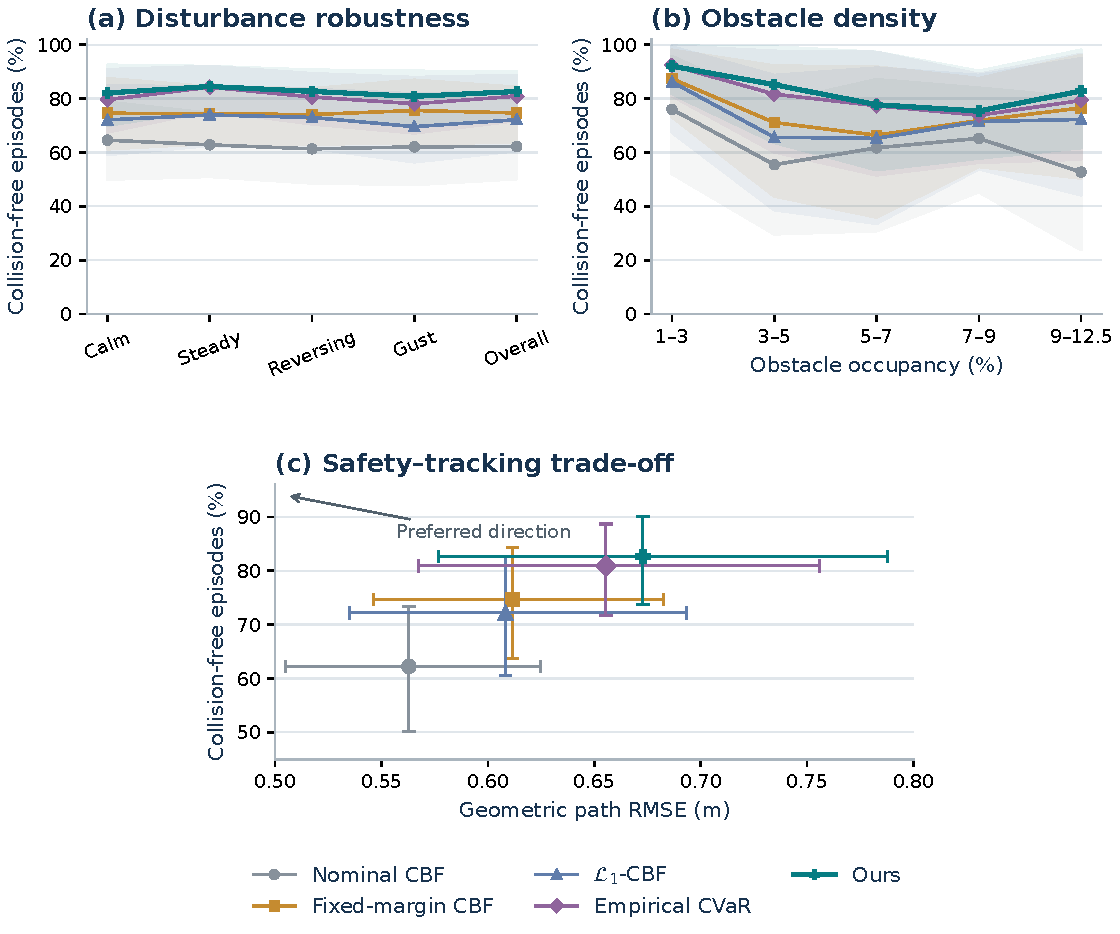
\includegraphics[width=\linewidth]{figures/results_robustness_panels.pdf}
\caption[Disturbance, density and safety--tracking comparisons]{Paired held-out evaluation. (a) Collision-free rate by disturbance. (b) Collision-free rate by obstacle occupancy. (c) Collision-free rate versus geometric path RMSE. Shaded bands and whiskers are hierarchical 95\% bootstrap intervals for one frozen policy; they do not measure variability across policy-training seeds.}
\label{fig:results_robustness_panels}
\end{figure}

The residual-tail filters maintain stronger collision avoidance across disturbance families and occupancy bands. The final panel makes the cost visible: the higher collision-free rate of Ours accompanies greater geometric path deviation. Its interval overlaps that of empirical CVaR, consistent with their close safety results. Appendix~\ref{app:rl_training} summarizes the PPO settings and policy-selection study.

\clearpage
\section{Sim2Sim Evaluation and the Sim2Real Gap}
\label{chap:sim2real}

\subsection{Simulation Performance and Physical Behavior}

A high success rate in simulation does not automatically translate into reliable flight. A policy can exploit its training environment, then struggle with different dynamics on a physical robot. Modeling errors are a central source of this sim2real gap~\cite{litPeng2018}. Imperfect sensing also changes what the robot knows about free space and approaching obstacles~\cite{extnavrl2025}.

The practical extension therefore moves beyond the simplified evaluation environment toward physics-based simulation. Isaac Sim provides rigid-body dynamics, collision models and simulated sensors in a common robotics platform~\cite{extisaacsim}. Its companion framework, Isaac Lab, supports large parallel learning workloads, making this ecosystem useful for both policy development and evaluation~\cite{extisaaclab}.

\begin{figure}[H]
\centering
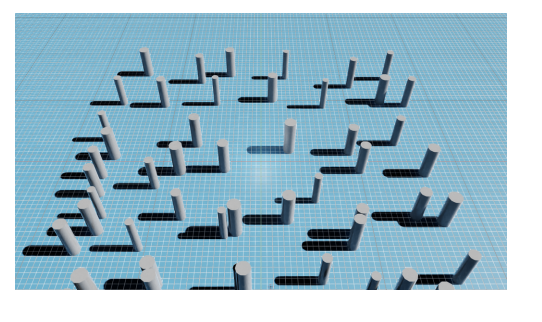
\includegraphics[width=.88\linewidth]{figures/sim2real_arena.png}
\caption[Obstacle arena for the practical navigation extension]{Overview of the obstacle arena used to illustrate the practical navigation extension. Closely spaced pillars create narrow passages and repeated avoidance decisions.}
\label{fig:sim2real_arena}
\end{figure}

This tests whether motion, sensing and collision geometry support the commands selected by the policy.

\clearpage
\subsection{Navigation with Local Perception}

Our sim2sim extension uses Isaac Sim and MuJoCo to examine navigation in richer physical environments. A preplanned A* route is smoothed with a B-spline, providing the reference path. The learned policy follows this reference and reacts when an unforeseen obstacle obstructs it, while the safety layer corrects the proposed command when needed.

The local map is built from simulated LiDAR observations with noise and missing returns, using sensing characteristics inspired by the Livox Mid-360. This changes the navigation problem: the controller must work with the space that has been observed, including gaps in that observation, instead of assuming complete obstacle geometry. The reference path supplies the overall route, and local perception supports the adjustments required during flight.

\begin{figure}[H]
\centering
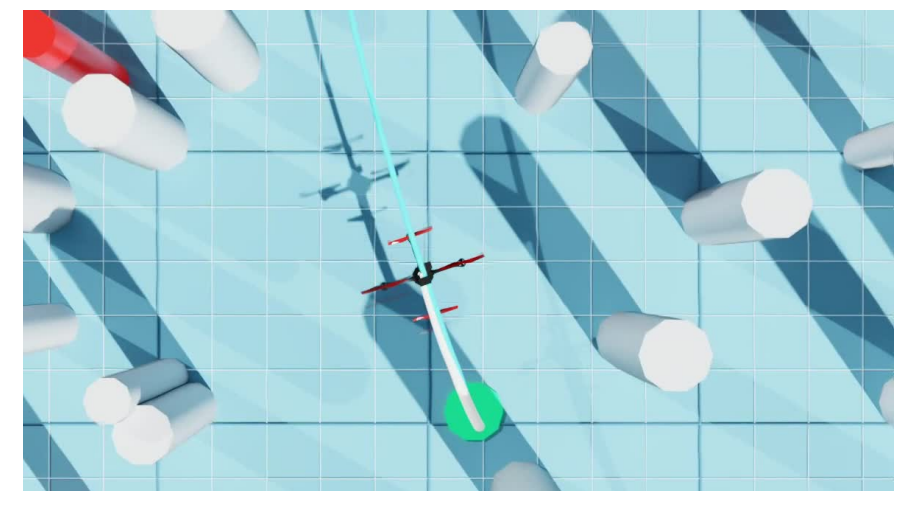
\includegraphics[width=\linewidth]{figures/sim2real_navigation.png}
\caption[Navigation among pillars with a reference path]{Close view of the navigation scene, showing the quadrotor, surrounding pillars, reference path and goal marker. The image illustrates the interaction between route following and local obstacle avoidance.}
\label{fig:sim2real_navigation}
\end{figure}

This stage complements disturbance evaluation by placing the navigation stack in a setting where motion and perception act together. It provides sim2sim evidence toward reducing the sim2real gap; physical flight remains a separate validation step.

\clearpage
\subsection{Comparison with NavRL}

NavRL is a relevant baseline for this setting. It learns UAV navigation with PPO, uses a velocity-obstacle-inspired safety shield and trains many simulated quadrotors in parallel with Isaac Sim. Its authors also demonstrate transfer to physical flight~\cite{extnavrl2025}. This combination of learned navigation, action correction and a physics-based training environment makes it a useful comparison for our practical extension.

Table~\ref{tab:sim2real_navrl} presents our extension benchmark, separately from the known-geometry evaluation in Section~\ref{sec:main_results}. Each scenario contains 72 static obstacles and a different number of dynamic obstacles. The entries compare mission success, collisions and the reported tracking error.

\begin{table}[H]
\centering
\caption[Practical navigation comparison with NavRL]{Practical navigation benchmark. S and D denote static and dynamic obstacles. Higher SR and lower CR and tracking error are preferred; bold values mark the better entry within each scenario.}
\label{tab:sim2real_navrl}
{\small\renewcommand{\arraystretch}{1.45}
\setlength{\tabcolsep}{5pt}
\begin{tabularx}{\linewidth}{@{}lYrrc@{}}
\toprule
\textbf{Scenario} & \textbf{Method} & \textbf{SR (\%)} & \textbf{CR (\%)} & \shortstack{\textbf{Tracking}\\\textbf{error (m)}}\\
\midrule
\multirow{2}{*}{72S + 12D} & Ours & \textbf{99.5} & \textbf{0.5} & \textbf{0.47}\\
 & NavRL & 74.1 & 15.4 & 1.23\\
\midrule
\multirow{2}{*}{72S + 20D} & Ours & \textbf{93.1} & \textbf{6.6} & \textbf{0.80}\\
 & NavRL & 61.6 & 35.1 & 1.15\\
\midrule
\multirow{2}{*}{72S + 40D} & Ours & \textbf{32.1} & \textbf{65.6} & 1.63\\
 & NavRL & 23.7 & 76.3 & \textbf{0.94}\\
\bottomrule
\end{tabularx}}
\end{table}

Ours achieves higher SR and lower CR in all three scenarios. With 12 dynamic obstacles, it reaches 99.5\% SR with 0.5\% CR. With 20, the success advantage is 31.5 percentage points and the collision rate is 28.5 points lower than NavRL. Tracking error is also lower in these first two settings.

With 40 dynamic obstacles, both methods deteriorate sharply. Ours retains higher SR and lower CR, but its tracking error is worse: 1.63\,m versus 0.94\,m. Tracking improves only in the first two scenarios. The extension's tracking-error aggregation is unspecified, so these values are not equated with the time-matched metric or geometric RMSE of Section~\ref{sec:main_results}.

\begingroup\setstretch{1.03}\setlength{\parskip}{0pt}
\chapter*{General Conclusion}
\phantomsection
\addcontentsline{toc}{chapter}{General Conclusion}
\markboth{General Conclusion}{General Conclusion}

Reliable robotic navigation must account for disturbances, imperfect observations and unexpected obstacles. This report has examined how reinforcement learning and control barrier functions address these challenges together: the policy provides task-directed behavior, while the safety filter corrects its actions according to the navigation constraints.

Our contribution introduces online disturbance adaptation into this architecture. An EMA-inspired observer estimates the disturbance, and a rolling window captures its remaining prediction errors. These residuals define an empirical distribution whose adverse tail is evaluated through a Wasserstein-robust CVaR margin. The resulting correction adapts to recent conditions while preserving the trained navigation policy. This provides a practical way to account for uncertainty without retraining the policy whenever the disturbance changes.

The evaluation shows that adaptation improves collision avoidance, at the cost of greater path deviation and more timeouts. In the main paired benchmark, Ours achieves a 73.6\% success rate, a 17.4\% collision rate and a 9.0\% timeout rate. Compared with the nominal filter, it maintains greater obstacle clearance but deviates further from the reference path. These results highlight the importance of assessing success, collisions, timeouts and tracking together.

The practical extension uses Isaac Sim and MuJoCo to examine navigation with richer physics and local perception. In the reported comparison with NavRL, Ours achieves higher success and lower collision rates in all three scenarios. Tracking error improves in the first two scenarios, while the most crowded dynamic setting remains difficult for both methods. This sim2sim evaluation is a step toward reducing the sim2real gap; physical flight is the next validation stage.

\section*{Future Work}
\phantomsection\addcontentsline{toc}{section}{Future Work}
Future work will focus on physical deployment and on reducing unnecessary path deviation while preserving the observed gains in collision avoidance.
Further evaluation will examine sensing and dynamics mismatch, observer and residual-window settings, and navigation among dense dynamic obstacles. These directions follow the limitations observed in the simulations.

\clearpage\endgroup

\appendix
\titleformat{\chapter}[display]{\normalfont\LARGE\bfseries\raggedright}{\large Appendix \thechapter}{8pt}{}

\chapter{RL Training and Policy Selection}
\label{app:rl_training}

\section{PPO Configuration}

Table~\ref{tab:ppo_specifications} records the PPO backbone settings used for navigation-policy training. The curriculum increases task difficulty while the optimization configuration remains fixed. GAE denotes generalized advantage estimation; its $\lambda$ parameter is distinct from the multiplier used by PPO-Lagrangian.

\begin{table}[H]
\centering
\caption{PPO backbone and training budget.}
\label{tab:ppo_specifications}
{\small\renewcommand{\arraystretch}{1.15}
\begin{tabularx}{\linewidth}{@{}Yl@{}}
\toprule
\textbf{Hyperparameter} & \textbf{Value}\\
\midrule
Hidden layers & $64,\;64$ units\\
Learning rate & $3\times10^{-4}$\\
Discount factor $\gamma$ & $0.99$\\
GAE parameter $\lambda$ & $0.95$\\
PPO clipping ratio & $0.20$\\
Entropy coefficient & $0.005$\\
Value-loss coefficient & $0.50$\\
Initial action log standard deviation & $-0.50$\\
Maximum gradient norm & $1.0$\\
Optimization epochs per update & $10$\\
Minibatches per epoch & $8$\\
Parallel environments & $4096$\\
Rollout length per environment & $258$ steps\\
Transitions per update & $1{,}056{,}768$\\
Training updates & $100$\\
Training transitions & $105{,}676{,}800$\\
Environment time step & $0.05$\,s\\
Training hardware & NVIDIA A100\\
\bottomrule
\end{tabularx}}
\end{table}

The interaction budget is aggregated across all parallel training environments.

\clearpage
\section{Policy-Selection Ablation}

The policy-selection study considers five RL regimes with five random seeds per regime, for 25 training runs. The comparison separates the effect of CBF action filtering from Lagrangian constraint handling and adversarial training.

\begin{table}[H]
\centering
\caption{RL regimes considered in the policy-selection study.}
\label{tab:rl_regimes}
{\small\renewcommand{\arraystretch}{1.35}
\begin{tabularx}{\linewidth}{@{}p{.37\linewidth}Yc@{}}
\toprule
\textbf{Regime} & \textbf{Training mechanism} & \textbf{Seeds}\\
\midrule
PPO & Reward-driven policy learning & 5\\
PPO+CBF & CBF correction of executed actions & 5\\
PPO-Lagrangian & Policy learning with a constraint multiplier & 5\\
PPO-Lagrangian+CBF & Constraint multiplier and CBF action filtering & 5\\
PPO+CBF+Adversarial & CBF filtering with an adversarial disturbance policy & 5\\
\bottomrule
\end{tabularx}}
\end{table}

\begin{figure}[H]
\centering
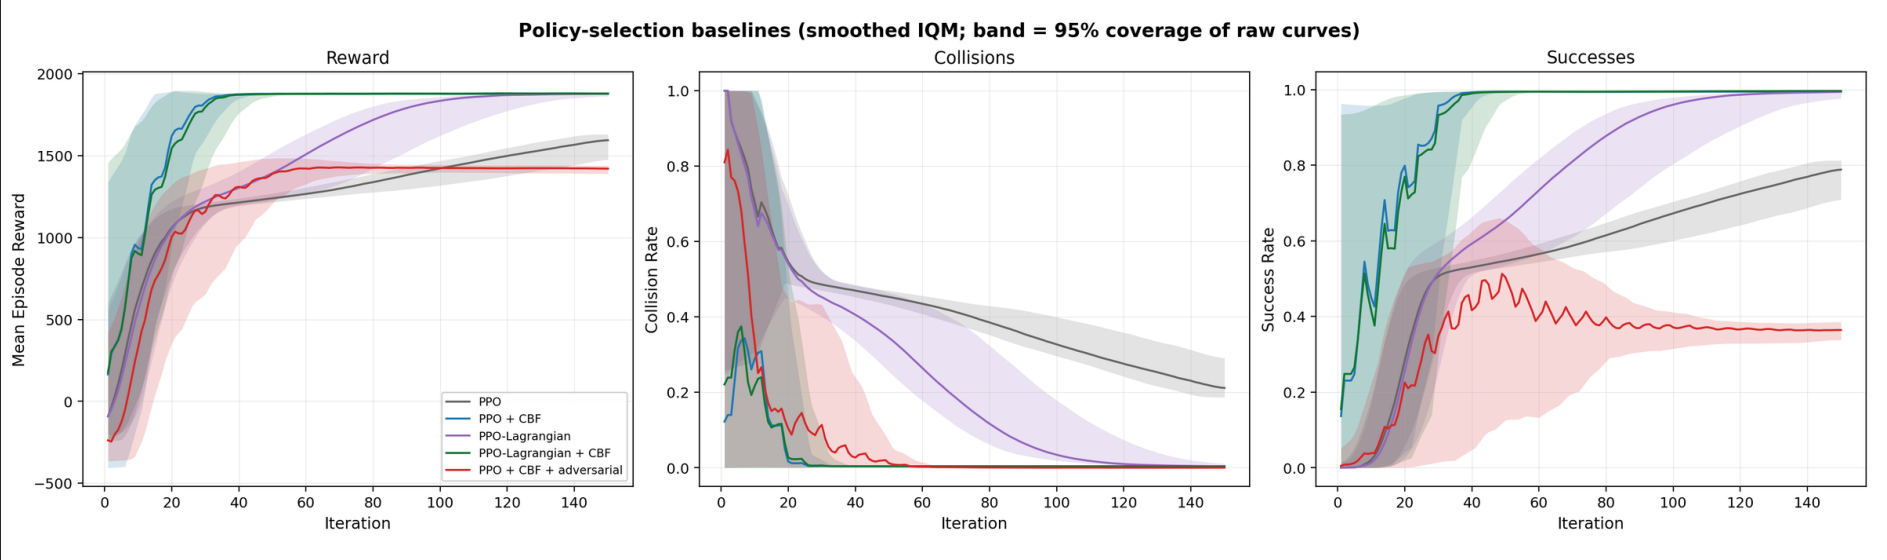
\includegraphics[width=\linewidth]{figures/rl_ablation_training.png}
\caption[Five-regime policy-selection training curves]{Reward, collision rate and success rate across the five RL regimes. Curves show the smoothed interquartile mean (IQM); shaded bands indicate 95\% coverage of raw curves, not confidence intervals.}
\label{fig:rl_ablation_training}
\end{figure}

Figure~\ref{fig:rl_ablation_training} shows that PPO+CBF and PPO-Lagrangian+CBF both reach high success and low collision rates early. PPO+CBF was retained for this favorable balance of learning efficiency and safety, with a simpler training objective that avoids multiplier updates and adversary optimization.

Learning efficiency here refers to progress over training interactions. The selected policy remains fixed in the main benchmark, where our contribution is the online adaptation of its downstream safety margin.

\chapter{Accepted WF-IoT Paper}
\label{app:wfiot}

\section{Publication Information}
Work carried out during this project led to a paper accepted at the IEEE World Forum on Internet of Things (WF-IoT).

\begin{description}[style=nextline,leftmargin=0pt,labelwidth=0pt,labelsep=0pt]
\item[Title] Wind-Aware Safe Navigation for Agile Quadrotors via Adaptive Barrier Filtering
\item[Authors] Salem Fradi, Hakim Ghazzai, Najmeddine Dhieb and Ahmed Eltawil
\item[Venue] IEEE World Forum on Internet of Things (WF-IoT)
\item[Status] Accepted
\end{description}

\section{Relationship to This Report}
The paper presents the disturbance-aware navigation architecture developed in this project: a learned navigation policy is combined with adaptive barrier filtering based on disturbance estimation and residual uncertainty. Chapters~\ref{ch:system} and~\ref{ch:contribution} explain the system model and proposed method, while Chapter~\ref{chap:results} presents the evaluation and discussion. This report provides the broader control and learning background, and Appendix~\ref{app:rl_training} documents the policy-training configuration and selection study.

\clearpage
\phantomsection\addcontentsline{toc}{chapter}{Bibliography}
{\small\setstretch{1.02}\setlength{\bibsep}{3pt}\bibliographystyle{IEEEtran}\bibliography{root_refs,literature_refs,theory_refs,extension_refs,wfiot_intro_refs}}
\end{document}

